% -*- Mode:TeX -*-

%% IMPORTANT: The official thesis specifications are available at:
%%            http://libraries.mit.edu/archives/thesis-specs/
%%
%%            Please verify your thesis' formatting and copyright
%%            assignment before submission. If you notice any
%%            discrepancies between these templates and the 
%%            MIT Libraries' specs, please let us know
%%            by e-mailing thesis@mit.edu

%% The documentclass options along with the pagestyle can be used to generate
%% a technical report, a draft copy, or a regular thesis. You may need to
%% re-specify the pagestyle after you \include cover.tex. For more
%% information, see the first few lines of mitthesis.cls. 

%\documentclass[12pt,vi,twoside]{mitthesis}
%%
%%  If you want your thesis copyright to you instead of MIT, use the
%%  ``vi'' option, as above.
%%
%\documentclass[12pt,twoside,leftblank]{mitthesis}
%%
%% If you want blank pages before new chapters to be labelled ``This
%% Page Intentionally Left Blank'', use the ``leftblank'' option, as
%% above. 

\documentclass[12pt]{mitthesis}
\usepackage{lgrind}
\pagestyle{drafthead}
%% These have been added at the request of the MIT Libraries, because
%% some PDF conversions mess up the ligatures.  -LB, 1/22/2014
\usepackage{cmap}
\usepackage[T1]{fontenc}
\usepackage{minted}
\usepackage{verbatim}
\usepackage{tikz}
\usemintedstyle{friendly}
\pagestyle{plain}

%% This bit allows you to either specify only the files which you wish to
%% process, or `all' to process all files which you \include.
%% Krishna Sethuraman (1990).

%\typein [\files]{Enter file names to process, (chap1,chap2 ...), or `all' to process all files:}
\def\all{all}
\ifx\files\all \typeout{Including all files.} \else %\typeout{Including only \files.} \includeonly{\files} \fi

\begin{document}

% -*-latex-*-
% 
% For questions, comments, concerns or complaints:
% thesis@mit.edu
% 
%
% $Log: cover.tex,v $
% Revision 1.9  2019/08/06 14:18:15  cmalin
% Replaced sample content with non-specific text.
%
% Revision 1.8  2008/05/13 15:02:15  jdreed
% Degree month is June, not May.  Added note about prevdegrees.
% Arthur Smith's title updated
%
% Revision 1.7  2001/02/08 18:53:16  boojum
% changed some \newpages to \cleardoublepages
%
% Revision 1.6  1999/10/21 14:49:31  boojum
% changed comment referring to documentstyle
%
% Revision 1.5  1999/10/21 14:39:04  boojum
% *** empty log message ***
%
% Revision 1.4  1997/04/18  17:54:10  othomas
% added page numbers on abstract and cover, and made 1 abstract
% page the default rather than 2.  (anne hunter tells me this
% is the new institute standard.)
%
% Revision 1.4  1997/04/18  17:54:10  othomas
% added page numbers on abstract and cover, and made 1 abstract
% page the default rather than 2.  (anne hunter tells me this
% is the new institute standard.)
%
% Revision 1.3  93/05/17  17:06:29  starflt
% Added acknowledgements section (suggested by tompalka)
% 
% Revision 1.2  92/04/22  13:13:13  epeisach
% Fixes for 1991 course 6 requirements
% Phrase "and to grant others the right to do so" has been added to 
% permission clause
% Second copy of abstract is not counted as separate pages so numbering works
% out
% 
% Revision 1.1  92/04/22  13:08:20  epeisach

% NOTE:
% These templates make an effort to conform to the MIT Thesis specifications,
% however the specifications can change. We recommend that you verify the
% layout of your title page with your thesis advisor and/or the MIT 
% Libraries before printing your final copy.
\title{Confidential and Crash-Safe Storage Systems}

\author{Atalay Mert Ileri}
% If you wish to list your previous degrees on the cover page, use the 
% previous degrees command:
%       \prevdegrees{A.A., Harvard University (1985)}
% You can use the \\ command to list multiple previous degrees
%       \prevdegrees{B.S., University of California (1978) \\
%                    S.M., Massachusetts Institute of Technology (1981)}
\department{Department of Electrical Engineering and Computer Science}

% If the thesis is for two degrees simultaneously, list them both
% separated by \and like this:
% \degree{Doctor of Philosophy \and Master of Science}
\degree{Doctor of Philosophy in Computer Science and Engineering}

% As of the 2007-08 academic year, valid degree months are September, 
% February, or June.  The default is June.
\degreemonth{June}
\degreeyear{1990}
\thesisdate{May 18, 1990}

%% By default, the thesis will be copyrighted to MIT.  If you need to copyright
%% the thesis to yourself, just specify the `vi' documentclass option.  If for
%% some reason you want to exactly specify the copyright notice text, you can
%% use the \copyrightnoticetext command.  
%\copyrightnoticetext{\copyright IBM, 1990.  Do not open till Xmas.}

% If there is more than one supervisor, use the \supervisor command
% once for each.
\supervisor{William J. Supervisor}{Associate Professor}

% This is the department committee chairman, not the thesis committee
% chairman.  You should replace this with your Department's Committee
% Chairman.
\chairman{Arthur C. Chairman}{Chairman, Department Committee on Graduate Theses}

% Make the titlepage based on the above information.  If you need
% something special and can't use the standard form, you can specify
% the exact text of the titlepage yourself.  Put it in a titlepage
% environment and leave blank lines where you want vertical space.
% The spaces will be adjusted to fill the entire page.  The dotted
% lines for the signatures are made with the \signature command.
\maketitle

% The abstractpage environment sets up everything on the page except
% the text itself.  The title and other header material are put at the
% top of the page, and the supervisors are listed at the bottom.  A
% new page is begun both before and after.  Of course, an abstract may
% be more than one page itself.  If you need more control over the
% format of the page, you can use the abstract environment, which puts
% the word "Abstract" at the beginning and single spaces its text.

%% You can either \input (*not* \include) your abstract file, or you can put
%% the text of the abstract directly between the \begin{abstractpage} and
%% \end{abstractpage} commands.

% First copy: start a new page, and save the page number.
\cleardoublepage
% Uncomment the next line if you do NOT want a page number on your
% abstract and acknowledgments pages.
% \pagestyle{empty}
\setcounter{savepage}{\thepage}
\begin{abstractpage}
% $Log: abstract.tex,v $
% Revision 1.1  93/05/14  14:56:25  starflt
% Initial revision
% 
% Revision 1.1  90/05/04  10:41:01  lwvanels
% Initial revision
% 
%
%% The text of your abstract and nothing else (other than comments) goes here.
%% It will be single-spaced and the rest of the text that is supposed to go on
%% the abstract page will be generated by the abstractpage environment.  This
%% file should be \input (not \include 'd) from cover.tex.
Lorem ipsum dolor sit amet, consectetur adipiscing elit. Nam quis neque et erat laoreet finibus at ac leo. Curabitur pellentesque, diam quis dignissim finibus, enim dui feugiat leo, nec porttitor sapien mi ac felis. Nam aliquam pretium nibh, quis dapibus dolor gravida sit amet. Cras porttitor dui quis elementum pulvinar. Nulla id pulvinar massa. Nullam ut diam non lorem venenatis faucibus. Vivamus lacus ante, pellentesque vitae nisl sit amet, bibendum facilisis purus.

\end{abstractpage}

% Additional copy: start a new page, and reset the page number.  This way,
% the second copy of the abstract is not counted as separate pages.
% Uncomment the next 6 lines if you need two copies of the abstract
% page.
% \setcounter{page}{\thesavepage}
% \begin{abstractpage}
% % $Log: abstract.tex,v $
% Revision 1.1  93/05/14  14:56:25  starflt
% Initial revision
% 
% Revision 1.1  90/05/04  10:41:01  lwvanels
% Initial revision
% 
%
%% The text of your abstract and nothing else (other than comments) goes here.
%% It will be single-spaced and the rest of the text that is supposed to go on
%% the abstract page will be generated by the abstractpage environment.  This
%% file should be \input (not \include 'd) from cover.tex.
Lorem ipsum dolor sit amet, consectetur adipiscing elit. Nam quis neque et erat laoreet finibus at ac leo. Curabitur pellentesque, diam quis dignissim finibus, enim dui feugiat leo, nec porttitor sapien mi ac felis. Nam aliquam pretium nibh, quis dapibus dolor gravida sit amet. Cras porttitor dui quis elementum pulvinar. Nulla id pulvinar massa. Nullam ut diam non lorem venenatis faucibus. Vivamus lacus ante, pellentesque vitae nisl sit amet, bibendum facilisis purus.

% \end{abstractpage}

\cleardoublepage

\section*{Acknowledgments}

This is the acknowledgements section. You should replace this with your
own acknowledgements.

%%%%%%%%%%%%%%%%%%%%%%%%%%%%%%%%%%%%%%%%%%%%%%%%%%%%%%%%%%%%%%%%%%%%%%
% -*-latex-*-

% Some departments (e.g. 5) require an additional signature page.  See
% signature.tex for more information and uncomment the following line if
% applicable.
% % -*- Mode:TeX -*-
%
% Some departments (e.g. Chemistry) require an additional cover page
% with signatures of the thesis committee.  Please check with your
% thesis advisor or other appropriate person to determine if such a 
% page is required for your thesis.  
%
% If you choose not to use the "titlepage" environment, a \newpage
% commands, and several \vspace{\fill} commands may be necessary to
% achieve the required spacing.  The \signature command is defined in
% the "mitthesis" class
%
% The following sample appears courtesy of Ben Kaduk <kaduk@mit.edu> and
% was used in his June 2012 doctoral thesis in Chemistry. 

\begin{titlepage}
\begin{large}
This doctoral thesis has been examined by a Committee of the Department
of Chemistry as follows:

\signature{Professor Jianshu Cao}{Chairman, Thesis Committee \\
   Professor of Chemistry}

\signature{Professor Troy Van Voorhis}{Thesis Supervisor \\
   Associate Professor of Chemistry}

\signature{Professor Robert W. Field}{Member, Thesis Committee \\
   Haslam and Dewey Professor of Chemistry}
\end{large}
\end{titlepage}


\pagestyle{plain}
\renewcommand{\ttdefault}{pxtt}

\newcommand{\red}{\color{red}}

\newcommand{\sys}{\textsc{DiskSec}\@\xspace}
\newcommand{\sfscq}{\textsc{SFSCQ}\@\xspace}

\newcommand{\URL}{\url}
\newcommand{\cc}[1]{\texttt{#1}}

\clubpenalty=10000
\widowpenalty=10000

\hyphenation{Fscq-Log}
\hyphenation{Certi-KOS}
\hyphenation{Applied-Unsync}
\hyphenation{i-node}
\hyphenation{Log-API}
\hyphenation{DFSCQ}
\hyphenation{SFSCQ}
\hyphenation{Sym-Diff}


\makeatletter
\def\PY@reset{\let\PY@it=\relax \let\PY@bf=\relax%
    \let\PY@ul=\relax \let\PY@tc=\relax%
    \let\PY@bc=\relax \let\PY@ff=\relax}
\def\PY@tok#1{\csname PY@tok@#1\endcsname}
\def\PY@toks#1+{\ifx\relax#1\empty\else%
    \PY@tok{#1}\expandafter\PY@toks\fi}
\def\PY@do#1{\PY@bc{\PY@tc{\PY@ul{%
    \PY@it{\PY@bf{\PY@ff{#1}}}}}}}
\def\PY#1#2{\PY@reset\PY@toks#1+\relax+\PY@do{#2}}

\expandafter\def\csname PY@tok@gd\endcsname{\def\PY@tc##1{\textcolor[rgb]{0.63,0.00,0.00}{##1}}}
\expandafter\def\csname PY@tok@gu\endcsname{\let\PY@bf=\textbf\def\PY@tc##1{\textcolor[rgb]{0.50,0.00,0.50}{##1}}}
\expandafter\def\csname PY@tok@gt\endcsname{\def\PY@tc##1{\textcolor[rgb]{0.00,0.27,0.87}{##1}}}
\expandafter\def\csname PY@tok@gs\endcsname{\let\PY@bf=\textbf}
\expandafter\def\csname PY@tok@gr\endcsname{\def\PY@tc##1{\textcolor[rgb]{1.00,0.00,0.00}{##1}}}
\expandafter\def\csname PY@tok@cm\endcsname{\let\PY@it=\textit\def\PY@tc##1{\textcolor[rgb]{0.25,0.50,0.50}{##1}}}
\expandafter\def\csname PY@tok@vg\endcsname{\def\PY@tc##1{\textcolor[rgb]{0.10,0.09,0.49}{##1}}}
\expandafter\def\csname PY@tok@mh\endcsname{\def\PY@tc##1{\textcolor[rgb]{0.40,0.40,0.40}{##1}}}
\expandafter\def\csname PY@tok@go\endcsname{\def\PY@tc##1{\textcolor[rgb]{0.53,0.53,0.53}{##1}}}
\expandafter\def\csname PY@tok@ge\endcsname{\let\PY@it=\textit}
\expandafter\def\csname PY@tok@vc\endcsname{\def\PY@tc##1{\textcolor[rgb]{0.10,0.09,0.49}{##1}}}
\expandafter\def\csname PY@tok@il\endcsname{\def\PY@tc##1{\textcolor[rgb]{0.40,0.40,0.40}{##1}}}
\expandafter\def\csname PY@tok@cs\endcsname{\let\PY@it=\textit\def\PY@tc##1{\textcolor[rgb]{0.25,0.50,0.50}{##1}}}
\expandafter\def\csname PY@tok@cp\endcsname{\def\PY@tc##1{\textcolor[rgb]{0.74,0.48,0.00}{##1}}}
\expandafter\def\csname PY@tok@gi\endcsname{\def\PY@tc##1{\textcolor[rgb]{0.00,0.63,0.00}{##1}}}
\expandafter\def\csname PY@tok@gh\endcsname{\let\PY@bf=\textbf\def\PY@tc##1{\textcolor[rgb]{0.00,0.00,0.50}{##1}}}
\expandafter\def\csname PY@tok@ni\endcsname{\let\PY@bf=\textbf\def\PY@tc##1{\textcolor[rgb]{0.60,0.60,0.60}{##1}}}
\expandafter\def\csname PY@tok@nl\endcsname{\def\PY@tc##1{\textcolor[rgb]{0.63,0.63,0.00}{##1}}}
\expandafter\def\csname PY@tok@nn\endcsname{\let\PY@bf=\textbf\def\PY@tc##1{\textcolor[rgb]{0.00,0.00,1.00}{##1}}}
\expandafter\def\csname PY@tok@no\endcsname{\def\PY@tc##1{\textcolor[rgb]{0.53,0.00,0.00}{##1}}}
\expandafter\def\csname PY@tok@na\endcsname{\def\PY@tc##1{\textcolor[rgb]{0.49,0.56,0.16}{##1}}}
\expandafter\def\csname PY@tok@nb\endcsname{\def\PY@tc##1{\textcolor[rgb]{0.00,0.50,0.00}{##1}}}
\expandafter\def\csname PY@tok@nc\endcsname{\let\PY@bf=\textbf\def\PY@tc##1{\textcolor[rgb]{0.00,0.00,1.00}{##1}}}
\expandafter\def\csname PY@tok@nd\endcsname{\def\PY@tc##1{\textcolor[rgb]{0.67,0.13,1.00}{##1}}}
\expandafter\def\csname PY@tok@ne\endcsname{\let\PY@bf=\textbf\def\PY@tc##1{\textcolor[rgb]{0.82,0.25,0.23}{##1}}}
\expandafter\def\csname PY@tok@nf\endcsname{\def\PY@tc##1{\textcolor[rgb]{0.00,0.00,1.00}{##1}}}
\expandafter\def\csname PY@tok@si\endcsname{\let\PY@bf=\textbf\def\PY@tc##1{\textcolor[rgb]{0.73,0.40,0.53}{##1}}}
\expandafter\def\csname PY@tok@s2\endcsname{\def\PY@tc##1{\textcolor[rgb]{0.73,0.13,0.13}{##1}}}
\expandafter\def\csname PY@tok@vi\endcsname{\def\PY@tc##1{\textcolor[rgb]{0.10,0.09,0.49}{##1}}}
\expandafter\def\csname PY@tok@nt\endcsname{\let\PY@bf=\textbf\def\PY@tc##1{\textcolor[rgb]{0.00,0.50,0.00}{##1}}}
\expandafter\def\csname PY@tok@nv\endcsname{\def\PY@tc##1{\textcolor[rgb]{0.10,0.09,0.49}{##1}}}
\expandafter\def\csname PY@tok@s1\endcsname{\def\PY@tc##1{\textcolor[rgb]{0.73,0.13,0.13}{##1}}}
\expandafter\def\csname PY@tok@kd\endcsname{\let\PY@bf=\textbf\def\PY@tc##1{\textcolor[rgb]{0.00,0.50,0.00}{##1}}}
\expandafter\def\csname PY@tok@sh\endcsname{\def\PY@tc##1{\textcolor[rgb]{0.73,0.13,0.13}{##1}}}
\expandafter\def\csname PY@tok@sc\endcsname{\def\PY@tc##1{\textcolor[rgb]{0.73,0.13,0.13}{##1}}}
\expandafter\def\csname PY@tok@sx\endcsname{\def\PY@tc##1{\textcolor[rgb]{0.00,0.50,0.00}{##1}}}
\expandafter\def\csname PY@tok@bp\endcsname{\def\PY@tc##1{\textcolor[rgb]{0.00,0.50,0.00}{##1}}}
\expandafter\def\csname PY@tok@c1\endcsname{\let\PY@it=\textit\def\PY@tc##1{\textcolor[rgb]{0.25,0.50,0.50}{##1}}}
\expandafter\def\csname PY@tok@kc\endcsname{\let\PY@bf=\textbf\def\PY@tc##1{\textcolor[rgb]{0.00,0.50,0.00}{##1}}}
\expandafter\def\csname PY@tok@c\endcsname{\let\PY@it=\textit\def\PY@tc##1{\textcolor[rgb]{0.25,0.50,0.50}{##1}}}
\expandafter\def\csname PY@tok@mf\endcsname{\def\PY@tc##1{\textcolor[rgb]{0.40,0.40,0.40}{##1}}}
\expandafter\def\csname PY@tok@mb\endcsname{\def\PY@tc##1{\textcolor[rgb]{0.40,0.40,0.40}{##1}}}
\expandafter\def\csname PY@tok@ss\endcsname{\def\PY@tc##1{\textcolor[rgb]{0.10,0.09,0.49}{##1}}}
\expandafter\def\csname PY@tok@sr\endcsname{\def\PY@tc##1{\textcolor[rgb]{0.73,0.40,0.53}{##1}}}
\expandafter\def\csname PY@tok@mo\endcsname{\def\PY@tc##1{\textcolor[rgb]{0.40,0.40,0.40}{##1}}}
\expandafter\def\csname PY@tok@kn\endcsname{\let\PY@bf=\textbf\def\PY@tc##1{\textcolor[rgb]{0.00,0.50,0.00}{##1}}}
\expandafter\def\csname PY@tok@gp\endcsname{\let\PY@bf=\textbf\def\PY@tc##1{\textcolor[rgb]{0.00,0.00,0.50}{##1}}}
\expandafter\def\csname PY@tok@kr\endcsname{\let\PY@bf=\textbf\def\PY@tc##1{\textcolor[rgb]{0.00,0.50,0.00}{##1}}}
\expandafter\def\csname PY@tok@s\endcsname{\def\PY@tc##1{\textcolor[rgb]{0.73,0.13,0.13}{##1}}}
\expandafter\def\csname PY@tok@kp\endcsname{\def\PY@tc##1{\textcolor[rgb]{0.00,0.50,0.00}{##1}}}
\expandafter\def\csname PY@tok@w\endcsname{\def\PY@tc##1{\textcolor[rgb]{0.73,0.73,0.73}{##1}}}
\expandafter\def\csname PY@tok@kt\endcsname{\def\PY@tc##1{\textcolor[rgb]{0.69,0.00,0.25}{##1}}}
\expandafter\def\csname PY@tok@ow\endcsname{\let\PY@bf=\textbf\def\PY@tc##1{\textcolor[rgb]{0.67,0.13,1.00}{##1}}}
\expandafter\def\csname PY@tok@sb\endcsname{\def\PY@tc##1{\textcolor[rgb]{0.73,0.13,0.13}{##1}}}
\expandafter\def\csname PY@tok@k\endcsname{\let\PY@bf=\textbf\def\PY@tc##1{\textcolor[rgb]{0.00,0.50,0.00}{##1}}}
\expandafter\def\csname PY@tok@se\endcsname{\let\PY@bf=\textbf\def\PY@tc##1{\textcolor[rgb]{0.73,0.40,0.13}{##1}}}
\expandafter\def\csname PY@tok@sd\endcsname{\let\PY@it=\textit\def\PY@tc##1{\textcolor[rgb]{0.73,0.13,0.13}{##1}}}

\def\PYZbs{\char`\\}
\def\PYZus{\char`\_}
\def\PYZob{\char`\{}
\def\PYZcb{\char`\}}
\def\PYZca{\char`\^}
\def\PYZam{\char`\&}
\def\PYZlt{\char`\<}
\def\PYZgt{\char`\>}
\def\PYZsh{\char`\#}
\def\PYZpc{\char`\%}
\def\PYZdl{\char`\$}
\def\PYZhy{\char`\-}
\def\PYZsq{\char`\'}
\def\PYZdq{\char`\"}
\def\PYZti{\char`\~}
% for compatibility with earlier versions
\def\PYZat{@}
\def\PYZlb{[}
\def\PYZrb{]}
\makeatother



\setlength{\abovedisplayskip}{0pt}
\setlength{\abovedisplayshortskip}{0pt}
\setlength{\belowdisplayskip}{0pt}
\setlength{\belowdisplayshortskip}{0pt}
\setlength{\jot}{0pt}

\setlength{\textfloatsep}{10pt plus 2pt minus 4pt}

\newcommand{\specfont}{\fontsize{9}{11}\selectfont}

%\numberwithin{equation}{section}

%\theoremstyle{definition}
\newtheorem{thm}{Theorem}
\newcommand{\thmautorefname}{Theorem}
%\newaliascnt{lemma}{thm}
%\newtheorem{lemma}[lemma]{Lemma}
%\aliascntresetthe{lemma}
%\newtheorem{lemma}{Lemma}[thm]
\newcommand{\lemmaautorefname}{Lemma}

\def\Snospace~{\S{}}
%\renewcommand*\sectionautorefname{\Snospace}
%\renewcommand{\subsectionautorefname}{\Snospace}
%\renewcommand{\subsubsectionautorefname}{\Snospace}

\newif\ifdraft\drafttrue
\newif\ifnotes\notestrue
\ifdraft\else\notesfalse\fi

% Define \XXX, \XXX[notes] and \XXX[author][notes]
\definecolor{xxxcolor}{rgb}{0.8,0,0}
\makeatletter
\long\def\XXX{\@ifnextchar[{\@XXX}{\@XXX[]}}
\long\def\@XXX[#1]{\@ifnextchar[{\@@@XXX{#1}}{\@@XXX{#1}}}
\ifnotes
% Show XXX comments
\long\def\@@XXX#1{{\color{xxxcolor} XXX #1}\xspace}
\long\def\@@@XXX#1[#2]{{\color{xxxcolor} XXX (#1) #2}\xspace}
\else
% Hide XXX comments
\long\def\@@XXX#1{\ignorespaces}
\long\def\@@@XXX#1[#2]{\ignorespaces}
\fi
\makeatother

%% Ensure ligatures (e.g., ``fine official flag'') can be copy/pasted from PDF.
\input{glyphtounicode}
\pdfgentounicode=1

%\bibpunct[: ]{[}{]}{,}{n}{XXX}{XXX}

\newcommand{\ind}{\hspace{0.5cm}}

\renewcommand{\topfraction}{0.95}
\renewcommand{\dbltopfraction}{0.95}
\renewcommand{\bottomfraction}{0.95}
\renewcommand{\textfraction}{0.05}
\renewcommand{\floatpagefraction}{0.95}
\renewcommand{\dblfloatpagefraction}{0.95}
\setcounter{topnumber}{10}
\setcounter{bottomnumber}{10}
\setcounter{totalnumber}{10}
\setcounter{dbltopnumber}{10}

%\tikzset{
  declare function={% in case of CVS which switches the arguments of atan2
    atan3(\a,\b)=ifthenelse(atan2(0,1)==90, atan2(\a,\b), atan2(\b,\a));},
  kinky cross radius/.initial=+.125cm,
  @kinky cross/.initial=+, kinky crosses/.is choice,
  kinky crosses/left/.style={@kinky cross=-},kinky crosses/right/.style={@kinky cross=+},
  kinky cross/.style args={(#1)--(#2)}{
    to path={
      let \p{@kc@}=($(\tikztotarget)-(\tikztostart)$),
          \n{@kc@}={atan3(\p{@kc@})+180} in
      -- ($(intersection of \tikztostart--{\tikztotarget} and #1--#2)!%
             \pgfkeysvalueof{/tikz/kinky cross radius}!(\tikztostart)$)
      arc [ radius     =\pgfkeysvalueof{/tikz/kinky cross radius},
            start angle=\n{@kc@},
            delta angle=\pgfkeysvalueof{/tikz/@kinky cross}180 ]
      -- (\tikztotarget)}}}


  % -*- Mode:TeX -*-
%% This file simply contains the commands that actually generate the table of
%% contents and lists of figures and tables.  You can omit any or all of
%% these files by simply taking out the appropriate command.  For more
%% information on these files, see appendix C.3.3 of the LaTeX manual. 
\tableofcontents
\newpage
\listoffigures
\newpage
\listoftables


\chapter{Introduction}

Explain the reason why there are two and how they compare to each other.



%% TODO: Short intro here
\subsection{Threat Model}
% Taken and tweaked from disksec
From the perspective of verification, we would like to have confidence
that the file system is secure purely based on the file system's security
specification.  This means that we have to treat the developer of the
file system with an adversarial mindset.  This subsumes all possible
bugs that a well-meaning but error-prone developer might introduce into
the implementation as well as any implementation that is designed to be exploited.

As a result, our threat model is that the adversary both develops the
file system and runs an adversarial application on top of the file system
in an attempt to obtain confidential file data.  However, the adversary
does provide a proof that their file-system implementation meets our
security specification.  The potential victim runs on top of the same
file system but sets their permissions so that the confidential files
are not accessible to the adversary's process.  Our goal is to ensure
that the security specification is so strong that it prevents leaks even
when the file-system developer is colluding with adversarial processes
running on top of the file system.

Our threat model is focused on proving that the file-system implementation has
no confidentiality bugs, rather than proving the absence of bugs in the
environment outside of the file system. Thus, we assume that our model
of how the file-system implementation executes is correct.  That is, we are not
concerned with bugs in unverified software or hardware outside of the file
system, or users mounting malicious disk images.  We do prove that
\texttt{mkfs} produces a correct image, but ensuring confidentiality on top of an
intentionally corrupted file system image is difficult, even without formal
verification. 

%%% Disksec doesn't reason about time. ConFrm reasons about it at coarse granularity.
%%% TODO: I will add these to their respective chapters

%We also do not reason about timing channels, as we do not model time.

%We only reasoning about time in a coarse granularity, 
%i.e. number of operations executed. Each operation having having different execution time 
%(e.g. a memory write is much faster than a disk write) is out of scope of this work.


% Taken from disksec
\subsection{Challenges}
\label{s:goal:chal}

The most difficult aspect of formally proving the security of a file system lies
in guaranteeing confidentiality.  This is difficult for several reasons.

\paragraph{Two-safety.}
First, proving confidentiality is more difficult than
proving functional correctness: as mentioned earlier, confidentiality
is a two-safety property.  Functional correctness is a one-safety
property because a violation of functional correctness can be demonstrated
by a single execution.  For instance, if an application wrote one byte to
a file and then read back a different byte, this single execution shows
that the file system is incorrect.  Thus, functional correctness
of a file system is a theorem that says that all executions meet the
spec (i.e., there are no such violations).  Integrity properties,
such as ensuring that one user cannot corrupt another user's data,
are an example of a one-safety functional-correctness property and can
be handled using standard verification techniques.

In contrast, demonstrating a violation of confidentiality requires
two executions, where the results observed by an adversary differ depending on
the secret data.
%% %% TODO: We don't do this though. Maybe find a better example for this?
For instance, consider a file system with block-level deduplication that
also exposes the number of free blocks.  An adversary who wants to
learn the contents of a victim's file could write their guess for the
victim's block into the adversary's own file and then check whether
the number of free blocks stayed the same or decreased.  If the file
system implemented deduplication across users, this attack allows an
adversary to learn whether their guess block was already present in the
file system, thus inferring whether the victim has that data.

In the above example, looking at a single execution does not allow one
to directly conclude that data was leaked, because the system appears
to be functioning correctly.  Determining that data is leaking requires
one to consider a pair of executions, in which the adversary performs
the same operations, but the confidential user data is different.
If these two executions produce different adversary-observable results,
the adversary is able to infer information about confidential data.

By stating confidentiality as a two-safety property, the above
deduplication example would violate confidentiality, and thus could not
appear in an implementation that was proven to achieve confidentiality.
Specifically, suppose the starting states of the two executions differed
in the contents of a confidential file, where in one execution the file
matched the adversary's guess and in the other execution it didn't match.
In this case, the number of free blocks returned by the adversary
would differ in the two executions, which would not be allowed by the
confidentiality definition.

\paragraph{Nondeterministic specifications.}
Another complication in proving confidentiality lies in the fact
that many specifications, including those in the file system, are
nondeterministic.  Some nondeterminism is unavoidable because file
systems must deal with crashes (e.g., due to power failure), which can
occur at any time.  Thus, it is impossible to
know what are the exact contents of the disk after a crash; the on-disk
state could reflect any prefix of the writes issued by the file system.
Modern disks complicate this situation even further by buffering writes
in memory inside the disk controller; as a result, the writes can be
made durable out-of-order, and the state of the disk after a crash might
reflect some out-of-order writes.  Even in the absence of crashes, the
file system implementation may want to use randomness (e.g., to randomize
directory hash tables), which makes the execution non-deterministic.

Other nondeterminism comes from specifications that hide irrelevant
details.  For instance, the inode allocator in the file system does
not specify which precise inode number will be returned; instead,
its specification simply states that it will return
\emph{some} inode number that is not already in use.

Any nondeterminism is a potential leak of confidential data.  The
nondeterministic specification of the block allocator from above does not
preclude the allocator from leaking confidential data, because it could,
in theory, choose the next inode number based on the confidential contents
of files, without violating its specification (i.e., still returning some
unused inode number).

Even the nondeterminism associated with the state of the disk
after a crash can be taken advantage of by an adversarial file-system
implementation to leak data.  For instance, a high-performance
file-system specification allows the file system to delay flushing data
to disk.  An adversarial implementation could choose whether to flush
data immediately or defer the flush based on one bit of confidential
data from a victim's file.  To take advantage of this, an adversary
could wait for the system to crash and, after the crash, check whether
any writes appear to have been lost.  If so, the adversary concludes
the file system must have deferred the writes, which would have only
happened if the confidential bit was zero.  This, in turn, can allow
the adversary to infer confidential bits.

\paragraph{Non-uniform outcome probabilities.}
Another possibility of leaking confidential data
arises because standard nondeterministic noninterference
captures what \emph{might} be possible, but an adversary may have
more precise information about the actual \emph{probabilities} of
different outcomes. A simple example of this weakness can be seen below: 

\begin{figure}[ht]
    \centering
\begin{verbatim}
if (random_bit() = 1)
  return secret_bit
else
  return random_bit()
\end{verbatim}
    \caption{Example of a noninterfering program that leaks information via return value frequencies}
    \label{fig:Frequency_Leaking_Program}
\end{figure}

This code leaks the secret bit 50\% of the time and outputs a random bit 50\% of the time. It is also important to note that it can output 0 or 1 independently of the secret value. This way, any (state, return) pair represents a successful execution. 

Let’s say that two states are equivalent if they are the same for their non secret parts. This makes all states equivalent to each other in our example. Since any pair of state and return value is a valid execution, it is possible to find another execution from a related state with same return value. Therefore, This implementation satisfies the nondeterministic noninterference definition. 

\begin{figure}[ht]
    \centering
    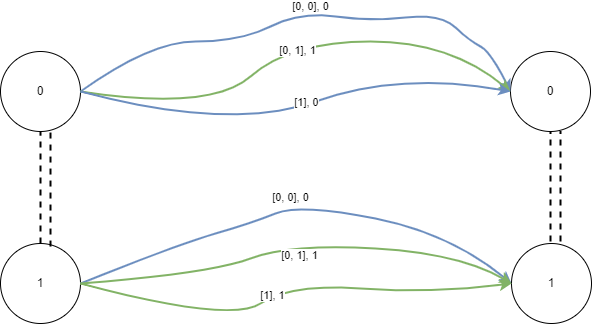
\includegraphics[scale=0.5]{templates/figures/matching-paths.png}
    \caption{Every execution matches with the execution of the same color.\\
    Numbers in brackets denote generated random bits. \\The number following the brackets denotes the return value.}
    \label{fig:NI_Matching_Paths}
\end{figure}

Although the above program satisfies the definition, the secret bit can be determined via the observed frequency of repeated calls. When we look at the frequencies of output values, we can see that they correlate with the value of the secret bit. \\

\begin{tabular}{| c | c | c |}
	\hline
	Secret bit & Output 0 \% & Output 1 \% \\
	\hline
	0 &	75\% & 25\% \\
	\hline
	1 &	25\% & 75\% \\
	\hline
\end{tabular}\\

Any adversary who can observe the output of the function sufficiently many times can infer the value of the secret bit with high confidence. These types of vulnerabilities are not limited to usage of randomization. They also manifest themselves when there are random events such as crashes that can affect the behavior of the system.


\paragraph{Indirect disclosure.}
Yet another complication with confidentiality is that an adversarial
file system might not immediately leak confidential data.  For example,
an adversarial file system may wait for a legitimate user to read
confidential data, at which point the file system would be allowed to
access this data, since it has to return it to the user.  However, in
addition to returning this data, an adversarial file system could also
stash away a copy of it, so that the adversary can later retrieve it.
For instance, the file system could change the order of entries in an
on-disk directory structure, or change the allocated inode numbers or
block numbers, based on the confidential data that it wants to leak.
Preventing this attack is difficult because the adversarial file system
appears to have legitimate access to the user's data when operating on
behalf of that user.

\paragraph{File-system complexity.}
Finally, file systems are complex software.  Linux ext4, for
instance, consists of approximately 50,000 lines of code.  Even the simple
verified DFSCQ file system consists of thousands of lines of executable
code~\cite{chen:dfscq}.  The proofs of functional correctness for DFSCQ
are already tens of thousands of lines of Coq code.  The complexity of
proving two-safety, which is a more challenging property, could easily
spiral out of control.

\chapter{Related Work}
\chapter{DiskSec}


\section{Specification: data noninterference}
\label{s:spec}

{\color{red} For some reason I am not happy with this part. I may rewrite this. }\\
%%%% Rewrite this to explain it is a form of relational noninterference.
To capture the notion of confidentiality in a file system, \sys
defines the notion of \emph{data noninterference}.  Loosely speaking,
data noninterference states that two executions are indistinguishable
with respect to specific confidential data (e.g., the contents of
a file).  Data noninterference allows an application to conclude that
an adversary cannot learn the contents of a file from the file system
but may be able to learn other information about the file (e.g., its
length, its creation time, the fact that it was created at all, etc.).
Furthermore, data noninterference does not place any restrictions on
application code, which captures the discretionary aspect of typical
file-system permissions.  This notion intuitively corresponds to the
security guarantees provided by Linux file systems.

%\begin{figure}[ht]
%  \centering
%    \begin{tikzpicture}[>=latex]

  \tikzstyle{state}=[circle, draw, minimum size=.8cm, node distance=2.5cm];
  \tikzstyle{ret}=[];
  \tikzstyle{exec}=[rectangle, rounded corners=3mm, opacity=0.2, fill=black, minimum width=8cm, minimum height=1.5cm];

  \tikzstyle{sim}=[<->, decorate, decoration={snake, pre length=2mm, post length=2mm, segment length=2mm}];
  \tikzstyle{syscall}=[->];
  \tikzstyle{sysret}=[->];
  \tikzstyle{retsim}=[<->, densely dotted, thick];

  \draw node (s0)  [state]              {$s_0$};
  \draw node (s'0) [state, below of=s0] {$s'_0$};

  \draw node (s1)  [state, right of=s0, xshift=1cm] {$s_1$};
  \draw node (s'1) [state, below of=s1] {$s'_1$};

  \draw node (s2)  [state, right of=s1, xshift=1cm] {$s_2$};
  \draw node (s'2) [state, below of=s2] {$s'_2$};

  \draw [sim] (s0) -- (s'0);
  \draw [sim] (s1) -- (s'1);
  \draw [sim] (s2) -- (s'2) {} node [pos=0.35, right] {$equivalent_{\mathrm{adv}}$};

  \draw [syscall] (s0) -- (s1)   node (s01)  [near start, below] {} node [midway, below] {$p_\mathrm{user}$};
  \draw [syscall] (s'0) -- (s'1) node (s'01) [near start, below] {} node [midway, below] {$p_\mathrm{user}$};

  \draw [ret] node (s01r)  [above of=s01,  xshift=1cm, yshift=-.2cm] {$r_0$};
  \draw [ret] node (s'01r) [above of=s'01, xshift=1cm, yshift=-.2cm] {$r'_0$};

  \draw [sysret] (s01.north)  to [out=0, in=225] (s01r);
  \draw [sysret] (s'01.north) to [out=0, in=225] (s'01r);

  \draw [syscall] (s1)  -- (s2)  node (s12)  [near start, below] {} node [midway, below] {$p_\mathrm{adv}$};
  \draw [syscall] (s'1) -- (s'2) node (s'12) [near start, below] {} node [midway, below] {$p_\mathrm{adv}$};
 
  \draw [ret] node (s12r)  [above of=s12,  xshift=1cm, yshift=-.2cm] {$r_1$};
  \draw [ret] node (s'12r) [above of=s'12, xshift=1cm, yshift=-.2cm] {$r'_1$};

  \draw [sysret] (s12.north)  to [out=0, in=225] (s12r);
  \draw [sysret] (s'12.north) to [out=0, in=225] (s'12r);
  \draw [retsim] (s12r) to [kinky cross=(s1)--(s2), kinky crosses=left] (s'12r);

  \draw node [exec, yshift=.25cm] at (s1.center) {};
  \draw node [exec, yshift=.25cm] at (s'1.center) {};

  %\draw [] node (sleg) [right of=s2] {$\cdot$};
  %\draw [] node (sleg') [right of=sleg, xshift=3mm] {$\cdot$};
  %\draw [syscall] (sleg) -- (sleg') {} node [midway, below] {$\mathrm{exec}$};

  %\draw [] node (rleg) [right of=s2, yshift=8mm] {};
  %\draw [] node (rleg') [below of=rleg, yshift=-3mm] {};
  %\draw [retsim] (rleg) -- (rleg') {} node [midway, right] {$=$};

  %\draw [] node (sleg2) [right of=s'2, yshift=8mm] {$\cdot$};
  %\draw [] node (sleg2') [below of=sleg2, yshift=-3mm] {$\cdot$};
  %\draw [sim] (sleg2) -- (sleg2') {} node [midway, right] {$equivalent_{\mathrm{adv}}$};

\end{tikzpicture}

%  \caption{Overview of \sys's approach to reasoning about confidentiality.}
%  \label{fig:approach}
%\end{figure}

\paragraph{Two-safety formulation.}
\sys formulates data noninterference in terms of two-safety, as shown
in \autoref{fig:approach}.  Specifically, data noninterference considers
two executions that run the same code but start from different states.  In
\autoref{fig:approach}, the executions are shown as horizontal transitions
between states, indicated by the gray outlines.  The executions
consist of a step by the user (running procedure $p_\mathrm{user}$,
corresponding to some system call) and then a step by the adversary
(running $p_\mathrm{adv}$, corresponding to some other system call).
Although \autoref{fig:approach} shows one particular pair of executions,
\sys's theorems consider all possible such pairs of executions.

The starting states in these two executions ($s_0$ and $s'_0$)
agree on all data visible to the adversary but could have
different contents of confidential files.  We call these two states
\emph{equivalent}$_\mathrm{adv}$, to indicate that they are equivalent
with respect to the adversary.  This equivalence is indicated by the
squiggly line in \autoref{fig:approach}.  The essence of data noninterference
is allowing the states to differ in the contents of confidential data
while requiring all other metadata (such as file length, directory order,
etc.) to remain the same.

{\color{red} Rewrite Ends Here. }\\
%%%%%%%%%%%%% Rewrite Ends Here %%%%%%%%%%%

The definition of data noninterference consists of two
requirements.  The first is \emph{state noninterference},
which requires that after every transition, the resulting states
remain \emph{equivalent}$_\mathrm{adv}$.  This is indicated in
\autoref{fig:approach} by the squiggly lines between $s_1$ and $s'_1$,
as well as between $s_2$ and $s'_2$.  This requirement ensures that
confidential data from $s_0$ and $s'_0$ does not suddenly become
accessible to the adversary in a subsequent state, and it addresses the
indirect-data-disclosure challenge.

The second requirement is \emph{return-value noninterference},
which requires that transitions by the adversary return exactly the
same values in both executions.  For example, \autoref{fig:approach}
shows that the adversary's $p_\mathrm{adv}$ returns $r_1$ in the top
execution and $r'_1$ in the bottom execution.  Return-value noninterference
requires that $r_1=r'_1$, as indicated by the dotted
arrow.  This prevents the adversary
from learning any confidential data, such as through collusion with an
adversarial file system.


\paragraph{Capturing file-system security.}

Achieving the two requirements from data noninterference ensures
that the adversary cannot obtain confidential data from the
file system.  This is because state noninterference maintains
\emph{equivalence}$_\mathrm{adv}$ regardless of what the adversary does, and any attempts by the adversary to observe
information will produce identical results, based on return-value
noninterference,
because they run in \emph{equivalent}$_\mathrm{adv}$ states.

The discretionary nature of data noninterference shows up in the fact
that legitimate users can obtain different results depending on the
confidential data.  For example, in \autoref{fig:approach}, the results
of the user's execution of $p_\mathrm{user}$, $r_0$ and $r'_0$, might be
different, because $p_\mathrm{user}$ could correspond to the user reading
a confidential file.  At this point, a user has the discretion to disclose this information
(e.g., by writing it to a public file).  Data noninterference does not
prevent this, by design, because it is attempting to model the standard
discretionary access control in a POSIX file system.


\paragraph{Defining return-value noninterference.}

\autoref{fig:two-safety-ret} presents \sys's definition of return-value
noninterference, in a simplified notation.  This definition relies on
the definition of \cc{exec}, which describes how procedures execute.
\cc{exec} takes four arguments: the procedure that is executing (\cc{p}),
the principal on whose behalf \cc{p} is running (\cc{u}), and the starting
state (\cc{st0}).
\cc{exec} returns two things: the outcome and an \emph{unseal trace},
which we describe later.
The outcome can be either \cc{Finished st' r}, indicating that the
procedure ended in state \cc{st'} and returned \cc{r}, or
\cc{Crashed st'}, indicating that the system crashed in state \cc{st'}.
The unseal traces are irrelevant for now and are used only as part of the
proof technique described in \autoref{s:proof}.
This definition also relies on a notion of two states being equivalent for
a particular principal, \cc{equivalent\_for\_principal}, which captures
the intuitive notion \emph{equivalent}$_\mathrm{adv}$ from above.

\begin{figure}[ht]
  \begin{BVerbatim}[commandchars=\\\{\},codes={\catcode`\$=3\catcode`\^=7\catcode`\_=8},fontsize=\footnotesize]
\PY{k+kn}{Definition} \PY{n}{equivalent\PYZus{}for\PYZus{}principal} \PY{n}{u} \PY{n}{st0} \PY{n}{st1} \PY{o}{:=}
  \PY{c}{(*}\PY{c}{ all parts of st0 and st1 that are accessible to}
\\[0.7\baselineskip]\PY{c}{     principal u are identical }\PY{c}{*)}\PY{o}{.}
\PY{k+kn}{Definition} \PY{n}{ret\PYZus{}noninterference} \PY{o}{`}\PY{o}{(}\PY{n}{p} \PY{o}{:} \PY{n}{proc} \PY{n}{T}\PY{o}{)} \PY{o}{:=}
  \PY{k}{forall} \PY{n}{u} \PY{n}{st0} \PY{n}{st0\PYZsq{}} \PY{n}{rand} \PY{n}{ret} \PY{n}{tr0} \PY{n}{st1}\PY{o}{,}
    \PY{n}{exec} \PY{n}{p} \PY{n}{u} \PY{n}{st0} \PY{n}{rand} \PY{o}{=}
        \PY{n}{Some} \PY{o}{(}\PY{n}{Finished} \PY{n}{st0\PYZsq{}} \PY{n}{ret}\PY{o}{,} \PY{n}{tr0}\PY{o}{)} \PY{o}{\PYZhy{}\PYZgt{}}
    \PY{n}{equivalent\PYZus{}for\PYZus{}principal} \PY{n}{u} \PY{n}{st0} \PY{n}{st1} \PY{o}{\PYZhy{}\PYZgt{}}
    \PY{k}{forall} \PY{n}{st1\PYZsq{}} \PY{n}{tr1}\PY{o}{,}
      \PY{n}{exec} \PY{n}{p} \PY{n}{u} \PY{n}{st1} \PY{n}{rand} \PY{o}{=}
          \PY{n}{Some} \PY{o}{(}\PY{n}{Finished} \PY{n}{st1\PYZsq{}} \PY{n}{ret\PYZsq{}}\PY{o}{,} \PY{n}{tr1}\PY{o}{)} \PY{o}{\PYZhy{}\PYZgt{}}
      \PY{n}{ret\PYZsq{}} \PY{o}{=} \PY{n}{ret}\PY{o}{.}
\end{BVerbatim}

  \caption{Definition of return-value noninterference, capturing that
    return values do not leak other users' confidential data.}
  \label{fig:two-safety-ret}
\end{figure}

The definition of return-value noninterference captures the intuition
about the adversary not being able to learn information about confidential
data: the return value obtained by the adversary by running some
code does not depend on the confidential data.  To make this precise,
\cc{ret\_noninterference} of procedure \cc{p} considers pairs of states,
\cc{st0} and \cc{st1}, which are equivalent as far as some principal
\cc{u} is concerned.  Here, \cc{u} is representing the adversary, and
confidential data is represented by the difference between \cc{st0} and
\cc{st1} that the adversary should not be able to observe.  If \cc{u}
runs procedure \cc{p} in state \cc{st0} and gets return value \cc{ret},
then it must also have been possible for the adversary to get the same
return value, \cc{ret}, if he ran \cc{p} in state \cc{st1} instead.


\paragraph{Defining state noninterference.}

\autoref{fig:two-safety-state} presents \sys's definition
of state noninterference, which complements return-value
noninterference.  This definition helps \sys deal with the indirect-disclosure
challenge from \autoref{s:goal:chal}.  This definition
considers two principals: a \cc{viewer} and a \cc{caller}.  The definition
intuitively says that, by running procedure \cc{p}, the caller will not
create any state differences observable to \cc{viewer}.

\begin{figure}[ht]
  \begin{BVerbatim}[commandchars=\\\{\},codes={\catcode`\$=3\catcode`\^=7\catcode`\_=8},fontsize=\footnotesize]
\PY{k+kn}{Definition} \PY{n}{equiv\PYZus{}state\PYZus{}for\PYZus{}principal} \PY{n}{u} \PY{n}{res0} \PY{n}{res1} \PY{o}{:=}
  \PY{k}{exists} \PY{n}{st0} \PY{n}{st1}\PY{o}{,}
    \PY{n}{equivalent\PYZus{}for\PYZus{}principal} \PY{n}{u} \PY{n}{st0} \PY{n}{st1} \PY{o}{/\PYZbs{}}
    \PY{o}{(}\PY{n}{res0} \PY{o}{=} \PY{n}{Crashed} \PY{n}{st0} \PY{o}{/\PYZbs{}} \PY{n}{res1} \PY{o}{=} \PY{n}{Crashed} \PY{n}{st1} \PY{o}{\PYZbs{}/}
     \PY{k}{exists} \PY{n}{v0} \PY{n}{v1}\PY{o}{,}
       \PY{n}{res0} \PY{o}{=} \PY{n}{Finished} \PY{n}{st0} \PY{n}{v0} \PY{o}{/\PYZbs{}}
\\[0.7\baselineskip]       \PY{n}{res1} \PY{o}{=} \PY{n}{Finished} \PY{n}{st1} \PY{n}{v1}\PY{o}{)}\PY{o}{.}
\PY{k+kn}{Definition} \PY{n}{state\PYZus{}noninterference} \PY{o}{`}\PY{o}{(}\PY{n}{p} \PY{o}{:} \PY{n}{proc} \PY{n}{T}\PY{o}{)} \PY{o}{:=}
  \PY{k}{forall} \PY{n}{viewer} \PY{n}{caller} \PY{n}{st0} \PY{n}{rand} \PY{n}{res0} \PY{n}{tr0} \PY{n}{st1}\PY{o}{,}
    \PY{n}{exec} \PY{n}{p} \PY{n}{caller} \PY{n}{st0} \PY{n}{rand} \PY{o}{=} \PY{n}{Some} \PY{o}{(}\PY{n}{res0}\PY{o}{,} \PY{n}{tr0}\PY{o}{)} \PY{o}{\PYZhy{}\PYZgt{}}
    \PY{n}{equivalent\PYZus{}for\PYZus{}principal} \PY{n}{viewer} \PY{n}{st0} \PY{n}{st1} \PY{o}{\PYZhy{}\PYZgt{}}
    \PY{k}{forall} \PY{n}{res1} \PY{n}{tr1}\PY{o}{,}
      \PY{n}{exec} \PY{n}{p} \PY{n}{caller} \PY{n}{st1} \PY{n}{rand} \PY{o}{=} \PY{n}{Some} \PY{o}{(}\PY{n}{res1}\PY{o}{,} \PY{n}{tr1}\PY{o}{)} \PY{o}{\PYZhy{}\PYZgt{}}
      \PY{n}{equiv\PYZus{}state\PYZus{}for\PYZus{}principal} \PY{n}{viewer} \PY{n}{res0} \PY{n}{res1}\PY{o}{.}
\end{BVerbatim}

  \caption{Definition of state noninterference, capturing that \cc{caller}
    does not indirectly disclose state to \cc{viewer}.}
  \label{fig:two-safety-state}
\end{figure}

More formally, \cc{state\_noninterference} considers two executions
by \cc{caller}, running the same procedure \cc{p}, with the same exact
arguments (encoded inside of \cc{p}).  If the caller runs \cc{p} in two
states that appear equivalent to \cc{viewer}, then the resulting states
in \cc{res0} and \cc{res1} will still appear equivalent to \cc{viewer}.
This definition includes the possibility of a crash while running \cc{p}.

\section{Proof approach: sealed blocks}
\label{s:proof}

Proving that every system call in a file system satisfies
\cc{ret\_noninterference} and \cc{state\_noninterference} would require
a proof that reasons about two executions, which is complex.  To reduce
proof effort, \sys introduces an implementation and proof approach
called \emph{sealed blocks}.  This approach factors out reasoning
about confidentiality of files from most of the file-system logic,
by reasoning about the confidentiality of disk blocks.  The intuition
behind this approach is threefold.  First, all confidential data lives
in file blocks.  Second, the file system itself rarely needs to look
inside of the file blocks.  Finally, permissions on files translate
directly into permissions on the underlying blocks comprising the file.

\begin{figure}[ht]
  \centering
  \scalebox{0.8}{
    \begin{tikzpicture}[>=latex]

  \tikzstyle{block}=[rectangle, draw, minimum height=0.5cm, minimum width=1.5cm, node distance=1cm];
  \tikzstyle{pblock}=[rectangle split, rectangle split parts=2, draw, minimum height=1cm, minimum width=1.5cm, node distance=1cm, align=left];
  \tikzstyle{sealed}=[fill=lightgray]

  \draw node (b0) [block] {data};
  \draw node (b1) [block, right of=b0, xshift=.5cm] {data};
  \draw node (b2) [block, right of=b1, xshift=.5cm] {data};
  \draw node [left of=b0, xshift=-2.5cm, anchor=west] {Real disk:};

  \draw node (p0) [pblock, above of=b0] {block \nodepart{second} perm};
  \draw node (p1) [pblock, right of=p0, xshift=.5cm] {block \nodepart{second} perm};
  \draw node (p2) [pblock, right of=p1, xshift=.5cm] {block \nodepart{second} perm};
  \draw node [left of=p0, xshift=-2.5cm, anchor=west] {Logical disk:};

  \draw [->] (b0) -- (p0);
  \draw [<-] (b2) -- (p2);

  \draw node (fs)
    [ rectangle, rounded corners=.2cm, draw,
      minimum width=6cm, minimum height=2cm,
      above of=p1, yshift=1.5cm ] {};
  \draw node [left of=fs, xshift=-4cm, anchor=west] {File system:};

  \draw node (fsp0) [pblock, sealed, above of=p0, yshift=1.5cm] {block \nodepart{second} perm};
  \draw node (fsp2) [pblock, sealed, above of=p2, yshift=1.5cm] {block \nodepart{second} perm};

  \draw [->] (p0.north) -- (fsp0.south) node [midway, left, align=right]
    {\phantom{x} \\ \em Read \\ \em block};
  \draw [->] (fsp2.south) -- (p2.north) node [midway, right, align=left]
    {\phantom{x} \\ \em Write \\ \em block};

  \draw node (w0) [block, above of=fsp0, yshift=2.25cm] {block};
  \draw node (w2) [block, above of=fsp2, yshift=2.25cm] {block};

  \draw [<-] (w0) -- (fsp0);
  \draw [<-] (fsp2) -- (w2);

  \draw node (fsread)
    [ rectangle, rounded corners=.2cm, draw, fill=white,
      minimum width=2.5cm, minimum height=1.5cm,
      above of=fs, yshift=1cm, xshift=-1.75cm ]
    {
      \begin{minipage}{2.5cm}
        \begin{Verbatim}[commandchars=\\\{\},codes={\catcode`\$=3\catcode`\^=7\catcode`\_=8},fontsize=\scriptsize]
\PY{k}{def} \PY{n+nf}{read}\PY{p}{(}\PY{o}{.}\PY{o}{.}\PY{o}{.}\PY{p}{)}\PY{p}{:}
  \PY{k}{if} \PY{n}{can\PYZus{}access}\PY{p}{(}\PY{p}{)}\PY{p}{:}
    \PY{n}{unseal}\PY{p}{(}\PY{n}{block}\PY{p}{)}
  \PY{o}{.}\PY{o}{.}\PY{o}{.}
\end{Verbatim}

      \end{minipage}
    };

  \draw node (fswrite)
    [ rectangle, rounded corners=.2cm, draw, fill=white,
      minimum width=2.5cm, minimum height=1.5cm,
      above of=fs, yshift=1cm, xshift=1.75cm ]
    {
      \begin{minipage}{2.5cm}
        \begin{Verbatim}[commandchars=\\\{\},codes={\catcode`\$=3\catcode`\^=7\catcode`\_=8},fontsize=\scriptsize]
\PY{k}{def} \PY{n+nf}{write}\PY{p}{(}\PY{o}{.}\PY{o}{.}\PY{o}{.}\PY{p}{)}\PY{p}{:}
  \PY{n}{perm} \PY{o}{=} \PY{n+nb}{file}\PY{o}{.}\PY{n}{acl}
  \PY{n}{seal}\PY{p}{(}\PY{n}{block}\PY{p}{,} \PY{n}{perm}\PY{p}{)}
  \PY{o}{.}\PY{o}{.}\PY{o}{.}
\end{Verbatim}

      \end{minipage}
    };

  \draw node [left of=fsread, xshift=-2.25cm, anchor=west, align=left] {Syscall \\ wrappers:};

\end{tikzpicture}

  }
  \caption{Overview of \sys's proof approach using sealed blocks.}
  \label{fig:sealing}
\end{figure}

\autoref{fig:sealing} presents an overview of \sys's block-sealing
approach.  There are three parts to the block-sealing approach.  The first
is to create a logical disk where every disk block is associated with a
\emph{permission}, which defines the set of principals that can access
this block.  Some permissions are public, indicating that the block is
accessible to anyone.  Other permissions might restrict access to some
users, indicating that this block is storing confidential file data.
\sys is agnostic to the specific choice of principals or permissions;
that is, all of \sys is parameterized over arbitrary types for
principals and permissions.  The logical disk is purely a proof strategy
and does not appear at runtime; the real disk, shown at the bottom of
\autoref{fig:sealing}, has no permissions.

The second part is a sealed-block abstraction, indicated by shaded
blocks in \autoref{fig:sealing}.  A sealed block represents the raw
block contents and the associated permission, but the file system cannot
directly access a sealed block's contents.  Instead, the file-system
implementation must explicitly call \cc{seal()} and \cc{unseal()} to
translate between sealed blocks and their raw contents.  These \cc{seal()}
and \cc{unseal()} functions are also purely part of the proof and do
not appear at runtime.

The code of the file system can read and write arbitrary blocks on
disk, but the result of a read is a sealed block that must be explicitly unsealed
if needed.  The file-system internals can unseal public blocks (e.g.,
containing allocator bitmaps or inodes) but cannot unseal private blocks.
This avoids the need to reason about the file-system implementation when
proving confidentiality, because the file-system implementation never
has access to confidential data.

The third part is the wrappers for system calls that handle confidential
data, namely, \cc{read()} and \cc{write()}.  These wrappers are responsible
for explicitly calling \cc{seal()} and \cc{unseal()} to translate between
the raw data seen by the user (on top of the system call) and the sealed
blocks that are handled in the rest of the file-system implementation.

\sys's sealed-block approach is a good fit for the challenges outlined in
\autoref{s:goal:chal}.  Specifically, there are very few places where a file
system must access the actual contents of a file's disk block---namely, in the
wrappers for the \cc{read()} and \cc{write()} syscalls.  As a result, most
specifications in a file system remain largely the same.  The key difference is
that the specifications promise that the procedure in question does not look
inside of any confidential blocks.  This means that any nondeterminism present
in the specification cannot be used to leak confidential data.

This approach allows file-system developers to avoid proving explicit
confidentiality theorems for most of the file system, but it still allows
\sys to conclude that confidentiality is not violated.  \sys provides a
theorem that proves two-safety for any file-system implementation that
correctly uses the sealed-block abstraction.  As a result, the
file-system developer need not reason about complex two-safety theorems
and can limit their reasoning to single executions.


\subsection{Formalizing sealed blocks}

To formally define \sys's sealed-block abstraction, \sys uses the
notion of a \emph{handle} to represent a sealed block.  \sys requires
the developer to perform two steps.  The first is to modify their code
to use the sealed-block abstraction: that is, to pass around handles
for blocks and to call \cc{seal()} and \cc{unseal()} as necessary.
The second is to prove that their code correctly follows the unsealing
rules.  This boils down to ensuring that sealed blocks are unsealed only
when the principal has appropriate permission for that block.

\sys models this by extending traditional Hoare logic to reason about
unseal operations.  Specifically, \sys builds on CHL~\cite{chen:fscq},
where functional correctness specifications are written in terms of
pre- and postconditions.  \sys, first, extends the execution semantics
(as we describe next) to produce an \emph{unseal trace} consisting of
unseal operations and, second, extends the specifications to require
that the unseal trace contain only allowed unseals.

We expect that systems built on top of \sys would often group multiple
blocks into a single object (e.g., multiple blocks comprising a single
file in a file system).  To help developers reason about all of these
blocks sharing the same permissions, \sys introduces the notion of
a \emph{domain}.  This is a layer of indirection between blocks and
permissions.  Specifically, sealed blocks point to a domain ID (e.g.,
an inode number in the case of a file system), and the domain in turn
specifies the permission for those blocks (e.g., the permission reflected
in the inode's data structure).



\paragraph{Execution model.}

\sys's execution model requires the implementation to be written in a
domain-specific language, based on CHL and implemented inside of Coq,
which provides several primitive operations.  These operations include
reading and writing the disk, manipulating sealed blocks by sealing and
unsealing, as well as others for sequencing computation, returning values,
flushing disk writes, etc.

\begin{figure}[ht]
  \begin{BVerbatim}[commandchars=\\\{\},codes={\catcode`\$=3\catcode`\^=7\catcode`\_=8},fontsize=\footnotesize]
\PY{k+kn}{Inductive} \PY{n}{nondet\PYZus{}decision} \PY{o}{:=}
\PY{o}{|} \PY{n}{RandomHandle} \PY{o}{(}\PY{n}{h}\PY{o}{:}\PY{n}{handle}\PY{o}{)}
\PY{c}{(*}\PY{c}{ Other types of non\PYZhy{}determinism omitted for space }\PY{c}{*)}
\\[0.7\baselineskip]\PY{o}{|} \PY{n}{CrashHere}\PY{o}{.}
\\[0.7\baselineskip]\PY{k+kn}{Definition} \PY{n}{oracle} \PY{o}{:=} \PY{k+kt}{list} \PY{n}{nondet\PYZus{}decision}\PY{o}{.}
\PY{k+kn}{Definition} \PY{n}{exec} \PY{o}{`}\PY{o}{(}\PY{n}{code}\PY{o}{:}\PY{n}{proc} \PY{n}{T}\PY{o}{)} \PY{o}{(}\PY{n}{u}\PY{o}{:}\PY{n}{Principal}\PY{o}{)} \PY{o}{(}\PY{n}{st}\PY{o}{:}\PY{n}{State}\PY{o}{)}
           \PY{o}{(}\PY{n}{rand}\PY{o}{:}\PY{n}{oracle}\PY{o}{)} \PY{o}{:} \PY{n}{option} \PY{o}{(}\PY{n}{result} \PY{n}{T} \PY{o}{*} \PY{n}{trace}\PY{o}{)} \PY{o}{:=}
  \PY{k}{match} \PY{n}{code}\PY{o}{,} \PY{n}{rand} \PY{k}{with}
  \PY{o}{|} \PY{n}{ChangePerm} \PY{o}{\PYZus{}} \PY{o}{\PYZus{}}\PY{o}{,} \PY{n}{CrashHere} \PY{o}{=\PYZgt{}} \PY{n}{None}
  \PY{o}{|} \PY{o}{\PYZus{}}\PY{o}{,} \PY{n}{CrashHere} \PY{o}{=\PYZgt{}} \PY{n}{Some} \PY{o}{(}\PY{n}{Crashed} \PY{n}{st}\PY{o}{,} \PY{n+nb+bp}{[]}\PY{o}{)}
  \PY{o}{|} \PY{n}{Read} \PY{n}{a}\PY{o}{,} \PY{n}{RandomHandle} \PY{n}{h} \PY{o}{=\PYZgt{}}
    \PY{k}{if} \PY{n}{addr\PYZus{}out\PYZus{}of\PYZus{}bounds} \PY{n}{st} \PY{n}{a} \PY{k}{then}
      \PY{n}{Some} \PY{o}{(}\PY{n}{Finished} \PY{n}{st} \PY{n}{hzero}\PY{o}{,} \PY{n+nb+bp}{[]}\PY{o}{)}
    \PY{k}{else} \PY{k}{if} \PY{n}{handle\PYZus{}used} \PY{n}{st} \PY{n}{h} \PY{k}{then}
      \PY{n}{None}
    \PY{k}{else}
      \PY{k}{let} \PY{n}{data} \PY{o}{:=} \PY{n}{disk\PYZus{}block\PYZus{}data} \PY{n}{st} \PY{n}{a} \PY{k}{in}
      \PY{k}{let} \PY{n}{dom}  \PY{o}{:=} \PY{n}{disk\PYZus{}block\PYZus{}dom}  \PY{n}{st} \PY{n}{a} \PY{k}{in}
      \PY{k}{let} \PY{n}{st\PYZsq{}} \PY{o}{:=} \PY{n}{install\PYZus{}handle} \PY{n}{st} \PY{n}{h} \PY{o}{(}\PY{n}{data}\PY{o}{,} \PY{n}{dom}\PY{o}{)} \PY{k}{in}
      \PY{n}{Some} \PY{o}{(}\PY{n}{Finished} \PY{n}{st\PYZsq{}} \PY{n}{h}\PY{o}{,} \PY{n+nb+bp}{[]}\PY{o}{)}
  \PY{o}{|} \PY{n}{Write} \PY{n}{a} \PY{n}{h}\PY{o}{,} \PY{o}{\PYZus{}} \PY{o}{=\PYZgt{}}
    \PY{k}{if} \PY{n}{handle\PYZus{}used} \PY{n}{st} \PY{n}{h} \PY{k}{then}
      \PY{k}{let} \PY{n}{data} \PY{o}{:=} \PY{n}{handle\PYZus{}data} \PY{n}{st} \PY{n}{h} \PY{k}{in}
      \PY{k}{let} \PY{n}{dom}  \PY{o}{:=} \PY{n}{handle\PYZus{}dom}  \PY{n}{st} \PY{n}{h} \PY{k}{in}
      \PY{k}{let} \PY{n}{st\PYZsq{}} \PY{o}{:=} \PY{n}{disk\PYZus{}block\PYZus{}write} \PY{n}{st} \PY{n}{a} \PY{o}{(}\PY{n}{data}\PY{o}{,} \PY{n}{dom}\PY{o}{)} \PY{k}{in}
      \PY{n}{Some} \PY{o}{(}\PY{n}{Finished} \PY{n}{st\PYZsq{}} \PY{n}{tt}\PY{o}{,} \PY{n+nb+bp}{[]}\PY{o}{)}
    \PY{k}{else}
      \PY{n}{Some} \PY{o}{(}\PY{n}{Finished} \PY{n}{st} \PY{n}{tt}\PY{o}{,} \PY{n+nb+bp}{[]}\PY{o}{)}
  \PY{c}{(*}\PY{c}{ Some transitions omitted for space reasons }\PY{c}{*)}
  \PY{o}{|} \PY{n}{Seal} \PY{n}{data} \PY{n}{dom}\PY{o}{,} \PY{n}{RandomHandle} \PY{n}{h} \PY{o}{=\PYZgt{}}
    \PY{k}{if} \PY{n}{handle\PYZus{}used} \PY{n}{st} \PY{n}{h} \PY{k}{then}
      \PY{n}{None}
    \PY{k}{else}
      \PY{k}{let} \PY{n}{st\PYZsq{}} \PY{o}{:=} \PY{n}{install\PYZus{}handle} \PY{n}{st} \PY{n}{h} \PY{o}{(}\PY{n}{data}\PY{o}{,} \PY{n}{dom}\PY{o}{)} \PY{k}{in}
      \PY{n}{Some} \PY{o}{(}\PY{n}{Finished} \PY{n}{st\PYZsq{}} \PY{n}{h}\PY{o}{,} \PY{n+nb+bp}{[]}\PY{o}{)}
  \PY{o}{|} \PY{n}{Unseal} \PY{n}{h}\PY{o}{,} \PY{o}{\PYZus{}} \PY{o}{=\PYZgt{}}
    \PY{k}{if} \PY{n}{handle\PYZus{}used} \PY{n}{st} \PY{n}{h} \PY{k}{then}
      \PY{k}{let} \PY{n}{data} \PY{o}{:=} \PY{n}{handle\PYZus{}data} \PY{n}{st} \PY{n}{h} \PY{k}{in}
      \PY{k}{let} \PY{n}{dom}  \PY{o}{:=} \PY{n}{handle\PYZus{}dom}  \PY{n}{st} \PY{n}{h} \PY{k}{in}
      \PY{k}{let} \PY{n}{perm} \PY{o}{:=} \PY{n}{domain\PYZus{}perm} \PY{n}{st} \PY{n}{dom} \PY{k}{in}
      \PY{n}{Some} \PY{o}{(}\PY{n}{Finished} \PY{n}{st} \PY{n}{data}\PY{o}{,} \PY{o}{[}\PY{n}{perm}\PY{o}{]}\PY{o}{)}
    \PY{k}{else}
      \PY{n}{Some} \PY{o}{(}\PY{n}{Finished} \PY{n}{st} \PY{n}{zero}\PY{o}{,} \PY{n+nb+bp}{[]}\PY{o}{)}
  \PY{o}{|} \PY{n}{ChangePerm} \PY{n}{dom} \PY{n}{newperm}\PY{o}{,} \PY{o}{\PYZus{}} \PY{o}{=\PYZgt{}}
    \PY{k}{let} \PY{n}{oldperm} \PY{o}{:=} \PY{n}{domain\PYZus{}perm} \PY{n}{st} \PY{n}{dom} \PY{k}{in}
    \PY{k}{let} \PY{n}{st\PYZsq{}} \PY{o}{:=} \PY{n}{domain\PYZus{}set\PYZus{}perm} \PY{n}{st} \PY{n}{dom} \PY{n}{newperm} \PY{k}{in}
    \PY{n}{Some} \PY{o}{(}\PY{n}{Finished} \PY{n}{st} \PY{n}{tt}\PY{o}{,} \PY{o}{[}\PY{n}{oldperm}\PY{o}{]}\PY{o}{)}
  \PY{o}{|} \PY{o}{\PYZus{}}\PY{o}{,} \PY{o}{\PYZus{}} \PY{o}{=\PYZgt{}} \PY{n}{None}
  \PY{k}{end}\PY{o}{.}
\end{BVerbatim}

  \caption{Execution semantics with logging of unseal operations.}
  \label{fig:exec}
\end{figure}

\autoref{fig:exec} shows a simplified version of \sys's execution
semantics.  The semantics are defined as a function that takes the
\cc{code} being executed (of type \cc{proc T}), the principal \cc{u}
running the operation (of type \cc{Principal}), and the starting state \cc{st}
(of type \cc{State}).  The function
produces a tuple consisting of a result (of type \cc{result T}) and
a trace of unsealed permissions (of type \cc{trace}).  The function
is allowed to return \cc{None} (as indicated by the \cc{option} type)
when there is no execution possible for the supplied randomness (e.g.,
the randomly chosen handle is already in use).

For example, consider the case that handles the \cc{Read a} operation,
which describes the execution of reading address \cc{a} from disk.
There are three sub-cases.  If the address is out of bounds, the \cc{Read}
returns a handle for a zero block, with an empty unseal trace.  If the handle
\cc{h} supplied by the randomness oracle is already in use, no execution
is possible.  Otherwise, the \cc{Read} initializes the new handle to
represent the block from address \cc{a}, with the block's domain ID, and
returns that handle, with an empty trace because no blocks were unsealed.

As another example, the \cc{Unseal h} operation produces a nonempty trace,
consisting of the permission of the sealed block whose handle \cc{h}
was unsealed, as long as the handle was valid (otherwise, \cc{Unseal}
returns zero).  Since the sealed block points to a domain ID, \cc{dom},
the semantics of \cc{Unseal} look up the corresponding permissions of
that domain.  One omitted rule handles concatenation of unseal traces when a
developer sequences one statement after another.

The \cc{ChangePerm dom newperm} operation allows the developer to
change permissions of a domain.  This operation is used in implementing
\cc{chown}.  The semantics of \cc{ChangePerm} modify the permission
associated with the domain, and produce an unseal trace containing the domain's
old permission, to reflect that data with that permission may have
been disclosed.  Since the domains are purely a proof construct,
\cc{ChangePerm} is a purely logical operation, which does not perform
any actions at runtime.

%%% Rewrite this to remove oracles
{\color{red} Rewrite this to remove oracles. }\\
Finally, \cc{exec} describes the possible crash behaviors of the system.
For example, the case for \cc{\_, CrashHere} states that it is possible to
crash in the starting state, regardless of what code was being executed,
if the randomness oracle tells us \cc{CrashHere}.  A combination
of other rules, not shown, allow crashing in the middle of a sequence of
operations.  The very first case, for \cc{ChangePerm \_ \_, CrashHere},
says that \cc{ChangePerm} cannot crash.  This reflects the fact that
\cc{ChangePerm} is a purely logical operation.

{\color{red} Rewrite Ends Here. }\\
%%%%%%%%%%%%%%%%%%%%%%%%%%%%%%%

\paragraph{Specification and verification of unseal rules.}

\sys requires developers to write specifications for each procedure, using
pre- and postconditions.  The postcondition describes how the procedure
modifies the state of the system, along with what must be true of the procedure's
return value, assuming that the precondition (a predicate over the system
state and the procedure's arguments) held at the start of the procedure.

To reason about what blocks a procedure might unseal, \sys augments
specification postconditions with requirements about the permissions
that appear in the unseal trace produced by the execution of the procedure.

\begin{figure}[ht]
  \begin{BVerbatim}[commandchars=\\\{\},codes={\catcode`\$=3\catcode`\^=7\catcode`\_=8},fontsize=\footnotesize]
\PY{k+kn}{Definition} \PY{n}{unseal\PYZus{}safe} \PY{o}{`}\PY{o}{(}\PY{n}{p} \PY{o}{:} \PY{n}{proc} \PY{n}{T}\PY{o}{)} \PY{o}{:=}
  \PY{k}{forall} \PY{n}{u} \PY{n}{st} \PY{n}{rand} \PY{n}{res} \PY{n}{tr}\PY{o}{,}
    \PY{n}{exec} \PY{n}{p} \PY{n}{u} \PY{n}{st} \PY{n}{rand} \PY{o}{=} \PY{n}{Some} \PY{o}{(}\PY{n}{res}\PY{o}{,} \PY{n}{tr}\PY{o}{)} \PY{o}{\PYZhy{}\PYZgt{}}
      \PY{k}{forall} \PY{n}{perm}\PY{o}{,}
        \PY{n}{In} \PY{n}{perm} \PY{n}{tr} \PY{o}{\PYZhy{}\PYZgt{}} \PY{n}{can\PYZus{}access} \PY{n}{u} \PY{n}{perm}\PY{o}{.}
\end{BVerbatim}

  \caption{Definition of unseal safety.}
  \label{fig:unseal-safety}
\end{figure}

\autoref{fig:unseal-safety} shows \sys's definition of unseal safety.
This definition says that procedure \cc{p} is ``unseal-safe'' if,
for every principal \cc{u} that runs this procedure and any starting
state \cc{st}, all permissions produced by this procedure in its unseal trace
\cc{tr} will be accessible to the calling principal.
%(This definition
%is simplified from \sys's actual implementation, because \sys's real
%definition appears in the postcondition of a more complex
%functional-correctness statement about all possible executions of \cc{p}.)
Proving unseal safety leads to a proof obligation for the file-system
developer---namely, proving that the implementation will unseal a block
only if the current principal has access to it.

File-system implementation code falls into three categories with respect
to proving unseal safety.  The first category are procedures that do not
invoke any \cc{Unseal} operations.  For these procedures, the resulting
unseal trace is always empty, and \sys is able to prove unseal safety without
any developer input.  Most of the file-system code falls in this category.

The second category are procedures that unseal public blocks.
Examples include accessing inodes, allocator bitmaps, directories, etc.
These procedures do produce unseal traces containing permissions, but all
of the permissions should be public.  Thus, the developer's job is to
show that these permissions are indeed public; once this is established,
showing that the current principal has access is straightforward (since
every principal has access to public permissions).

To prove that the permissions are indeed public, the developer
relies on representation invariants of the file system.  For example, the
invariant for the block allocator states that all of the bitmap blocks
are public. The developer can assume this invariant within any implementation of
the block allocator API, which helps her prove that the block in question has
public permissions. In turn the developer must prove that the invariant is
preserved by every procedure (including across crashes and recovery), and show
that it is established at initialization time by \cc{mkfs}.

The final category are procedures that unseal private blocks.  In a
file system, this happens only in the implementation of the \cc{read}
system call, which returns file data to the caller.  The implementation (wrapper)
of the \cc{read} system call contains explicit code to obtain the current
principal, get the file's ACL (access control list) from the inode, and
compare them.  The developer's job is to prove that this code correctly
performs the permission check.  This proof typically relies on the
file's representation invariant, which asserts that every file block
is tagged with a permission matching the ACL stored in the inode.

\begin{figure}[ht]
  \begin{BVerbatim}[commandchars=\\\{\},codes={\catcode`\$=3\catcode`\^=7\catcode`\_=8},fontsize=\footnotesize]
\PY{k+kn}{Definition} \PY{n}{unseal\PYZus{}public} \PY{o}{`}\PY{o}{(}\PY{n}{p} \PY{o}{:} \PY{n}{proc} \PY{n}{T}\PY{o}{)} \PY{o}{:=}
  \PY{k}{forall} \PY{n}{u} \PY{n}{st} \PY{n}{rand} \PY{n}{res} \PY{n}{tr}\PY{o}{,}
    \PY{n}{exec} \PY{n}{p} \PY{n}{u} \PY{n}{st} \PY{n}{rand} \PY{o}{=} \PY{n}{Some} \PY{o}{(}\PY{n}{res}\PY{o}{,} \PY{n}{tr}\PY{o}{)} \PY{o}{\PYZhy{}\PYZgt{}}
      \PY{k}{forall} \PY{n}{perm}\PY{o}{,}
        \PY{n}{In} \PY{n}{perm} \PY{n}{tr} \PY{o}{\PYZhy{}\PYZgt{}} \PY{n}{perm} \PY{o}{=} \PY{n}{Public}\PY{o}{.}
\end{BVerbatim}

  \caption{Definition of \cc{unseal\_public}.}
  \label{fig:unseal-public}
\end{figure}

\sys also provides a stronger version of unseal-safety, as shown in
\autoref{fig:unseal-public}, called \cc{unseal\_public}.  A procedure
satisfies this definition if all of its code falls in the first two
categories above: that is, the procedure either unseals no blocks
at all or unseals only public blocks.  This alternative definition is
strictly stronger than unseal-safety; any procedure that satisfies
\cc{unseal\_public} is also unseal-safe.  The distinction between these
two notions will help the developer prove noninterference theorems,
as we will describe in \autoref{s:design:prove}.

\paragraph{Crashes.}

\sys's approach naturally extends to reasoning about crashes.
\sys's disk-crash model builds on the CHL model of disk
crashes~\cite{chen:fscq, chen:dfscq}.  After a crash, disk blocks can
be updated nondeterministically, as in CHL, based on outstanding writes
that are in the disk's write buffer but have not been flushed yet to
durable storage.  However, domains always follow the
data for pending writes; that is, logically, the content of the disk
block is updated atomically together with its domain ID\@.

All handles are invalidated after a crash, to model the fact that the
computer reboots and all in-memory state is lost.  All recovery code,
such as log replay or \cc{fsck}, is proven correct in \sys, which means
that it must follow the same block-sealing rules as the rest of the
file-system code.  This ensures that no data can be disclosed by the
recovery code.


\subsection{Proving noninterference}
\label{s:design:prove}

To help the developer prove the two types of noninterference, \sys
provides helper theorems.  \autoref{fig:unseal-to-ret} shows the first
one, which proves return-value noninterference based on unseal-safety.
\sys proves this theorem by considering all operations performed by
procedure \cc{p}.  Each operation must produce the same result in the
two executions being considered, since the states are equivalent for the
principal in question, \cc{u}.  The only way in which the executions
could differ is if they unsealed a block that was not accessible
to \cc{u}.  However, \cc{unseal\_safe} says that this is impossible.
This theorem also applies to procedures that are \cc{unseal\_public},
since that notion is strictly stronger than \cc{unseal\_safe}.

\begin{figure}[ht]
  \begin{BVerbatim}[commandchars=\\\{\},codes={\catcode`\$=3\catcode`\^=7\catcode`\_=8},fontsize=\footnotesize]
\PY{k+kn}{Theorem} \PY{n}{unseal\PYZus{}safe\PYZus{}to\PYZus{}ret\PYZus{}noninterference} \PY{o}{:}
  \PY{k}{forall} \PY{o}{`}\PY{o}{(}\PY{n}{p} \PY{o}{:} \PY{n}{proc} \PY{n}{T}\PY{o}{)}\PY{o}{,}
    \PY{n}{unseal\PYZus{}safe} \PY{n}{p} \PY{o}{\PYZhy{}\PYZgt{}} \PY{n}{ret\PYZus{}noninterference} \PY{n}{p}\PY{o}{.}
\end{BVerbatim}

  \caption{Theorem connecting unseal-safety to return-value noninterference.}
  \label{fig:unseal-to-ret}
\end{figure}

\autoref{fig:unseal-to-state} shows the second theorem provided by \sys,
for reasoning about state noninterference.  This theorem requires that
the procedure satisfy the stronger definition, \cc{unseal\_public}, to
ensure state noninterference.  The intuition for why this theorem is
true lies in the fact that a procedure that unseals only public blocks
cannot obtain any confidential data in the first place.  As a result,
this procedure's execution will be identical regardless of the contents of
confidential blocks, and thus the state after this procedure's execution
will remain equivalent from the adversary's point of view.  \sys proves
this theorem formally in Coq.

\begin{figure}[ht]
  \begin{BVerbatim}[commandchars=\\\{\},codes={\catcode`\$=3\catcode`\^=7\catcode`\_=8},fontsize=\footnotesize]
\PY{k+kn}{Theorem} \PY{n}{unseal\PYZus{}public\PYZus{}to\PYZus{}state\PYZus{}noninterference} \PY{o}{:}
  \PY{k}{forall} \PY{o}{`}\PY{o}{(}\PY{n}{p} \PY{o}{:} \PY{n}{proc} \PY{n}{T}\PY{o}{)}\PY{o}{,}
    \PY{n}{unseal\PYZus{}public} \PY{n}{p} \PY{o}{\PYZhy{}\PYZgt{}} \PY{n}{state\PYZus{}noninterference} \PY{n}{p}\PY{o}{.}
\end{BVerbatim}

  \caption{Theorem connecting \cc{unseal\_public} to state noninterference.}
  \label{fig:unseal-to-state}
\end{figure}

\sys does not provide a general-purpose theorem for reasoning about state
noninterference for procedures that satisfy only the weaker notion of
unseal-safety (i.e., that unseal private blocks), such as the \cc{read()}
system call.  Such procedures can indirectly disclose data as
described in \autoref{s:goal:chal} to legitimately unseal confidential
data on behalf of the currently executing principal but then stash a
copy of it.  It is up to the file-system developer to prove the state
noninterference of those procedures.  \autoref{s:fs} will discuss in
more detail how \sfscq structures its implementation to simplify these
proofs; in the case of \sfscq, the only system call that requires this
type of reasoning is \cc{read}.

\chapter{Case study: File system}
\label{s:fs}

To evaluate whether Disksec allows specifying and proving confidentiality
for a file system, we applied Disksec to the DFSCQ verified file system,
producing the SFSCQ verified secure file system, as described below.


\subsection{Specifying security}

The core specification of confidentiality for SFSCQ lies in the
write system call, as shown in XXX.  This
specification says that the \emph{data} argument to the {write}
system call remains confidential.  This is stated formally by
considering two different executions, starting from the same
state {st}, where different data ({data0} and {data1})
are written to the same offset {off} of the same file {f}.
The results, {res0} and {res1}, must be equivalent for any
adversary {adv} that does not have permission to access file {f}.
Since {equivalent\_state\_for\_principal} considers both crashing and
noncrashing executions, this definition ensures that the data passed to
{write} remains confidential regardless of whether the system crashes
or not.

%\begin{figure}[ht]
%  \begin{BVerbatim}[commandchars=\\\{\},codes={\catcode`\$=3\catcode`\^=7\catcode`\_=8},fontsize=\footnotesize]
\PY{k+kn}{Theorem} \PY{n}{write\PYZus{}confidentiality} \PY{o}{:}
  \PY{k}{forall} \PY{n}{f} \PY{n}{off} \PY{n}{data0} \PY{n}{data1} \PY{n}{caller} \PY{n}{st} \PY{n}{rand} \PY{n}{res0} \PY{n}{tr0}\PY{o}{,}
    \PY{n}{exec} \PY{o}{(}\PY{n}{write} \PY{n}{f} \PY{n}{off} \PY{n}{data0}\PY{o}{)} \PY{n}{caller} \PY{n}{st} \PY{n}{rand} \PY{o}{=}
                               \PY{n}{Some} \PY{o}{(}\PY{n}{res0}\PY{o}{,} \PY{n}{tr0}\PY{o}{)} \PY{o}{\PYZhy{}\PYZgt{}}
      \PY{k}{exists} \PY{n}{res1} \PY{n}{tr1}\PY{o}{,}
        \PY{n}{exec} \PY{o}{(}\PY{n}{write} \PY{n}{f} \PY{n}{off} \PY{n}{data1}\PY{o}{)} \PY{n}{caller} \PY{n}{st} \PY{n}{rand} \PY{o}{=}
                               \PY{n}{Some} \PY{o}{(}\PY{n}{res1}\PY{o}{,} \PY{n}{tr1}\PY{o}{)} \PY{o}{/\PYZbs{}}
        \PY{k}{forall} \PY{n}{adv}\PY{o}{,}
          \PY{o}{\PYZti{}} \PY{n}{can\PYZus{}access} \PY{n}{adv} \PY{o}{(}\PY{n}{file\PYZus{}perm} \PY{n}{st} \PY{n}{f}\PY{o}{)} \PY{o}{\PYZhy{}\PYZgt{}}
          \PY{n}{equiv\PYZus{}state\PYZus{}for\PYZus{}principal} \PY{n}{adv} \PY{n}{res0} \PY{n}{res1}\PY{o}{.}
\end{BVerbatim}

%  \caption{Confidentiality specification for the {write} system call.}
%  \label{fig:writespec}
%\end{figure}

The other part of the security specification lies in the {chown}
system call, which changes the permissions on existing files, and thus
affects what data is or is not confidential.  Because {chown} can
disclose the contents of a previously confidential file, the standard
definition of state non-interference from XXX
does not hold for {chown}.  Specifically, even if an adversary
{viewer} could not distinguish states {st0} and {st1} before some
{caller} executed {chown}, the adversary may nonetheless be able
to distinguish {st0} and {st1} after the {chown} runs because
the adversary may now have permission to read the previously confidential
file.

The security of {chown} is defined by a specialized version of
state non-interference, which considers three cases.  The first case
is that the adversary {viewer} does not have access to the file
after the {chown} (i.e., is not the new owner).
In this case, state non-interference holds.
The second case is that the adversary {viewer} does gain access to
the file after {chown} (i.e., is the new owner),
but the file had the same contents in the
two executions (i.e., in states {st0} and {st1}).  In this case,
state non-interference holds as well.  Finally, the adversary {viewer}
may gain access to the file \emph{and} the files had different contents in
the two executions.  In this case, state non-interference does not apply.
XXX summarizes this formally.

%\begin{figure}[ht]
%  \begin{BVerbatim}[commandchars=\\\{\},codes={\catcode`\$=3\catcode`\^=7\catcode`\_=8},fontsize=\footnotesize]
\PY{k+kn}{Definition} \PY{n}{chown\PYZus{}state\PYZus{}noninterference} \PY{n}{f} \PY{n}{new\PYZus{}owner} \PY{o}{:=}
  \PY{k}{forall} \PY{n}{viewer} \PY{n}{caller} \PY{n}{st0} \PY{n}{rand} \PY{n}{res0} \PY{n}{tr0} \PY{n}{st1}\PY{o}{,}
    \PY{n}{exec} \PY{o}{(}\PY{n}{chown} \PY{n}{f} \PY{n}{new\PYZus{}owner}\PY{o}{)} \PY{n}{caller} \PY{n}{st0} \PY{n}{rand} \PY{o}{=}
                                \PY{n}{Some} \PY{o}{(}\PY{n}{res0}\PY{o}{,} \PY{n}{tr0}\PY{o}{)} \PY{o}{\PYZhy{}\PYZgt{}}
    \PY{o}{(} \PY{n}{file\PYZus{}data} \PY{n}{st0} \PY{n}{f} \PY{o}{=} \PY{n}{file\PYZus{}data} \PY{n}{st1} \PY{n}{f} \PY{o}{\PYZbs{}/}
      \PY{n}{viewer} \PY{o}{\PYZlt{}}\PY{o}{\PYZgt{}} \PY{n}{new\PYZus{}owner} \PY{o}{)} \PY{o}{\PYZhy{}\PYZgt{}}
    \PY{n}{equivalent\PYZus{}for\PYZus{}principal} \PY{n}{viewer} \PY{n}{st0} \PY{n}{st1} \PY{o}{\PYZhy{}\PYZgt{}}
      \PY{k}{exists} \PY{n}{res1} \PY{n}{tr1}\PY{o}{,}
        \PY{n}{exec} \PY{o}{(}\PY{n}{chown} \PY{n}{f} \PY{n}{new\PYZus{}owner}\PY{o}{)} \PY{n}{caller} \PY{n}{st1} \PY{n}{rand} \PY{o}{=}
                                \PY{n}{Some} \PY{o}{(}\PY{n}{res1}\PY{o}{,} \PY{n}{tr1}\PY{o}{)} \PY{o}{/\PYZbs{}}
        \PY{n}{equiv\PYZus{}state\PYZus{}for\PYZus{}principal} \PY{n}{viewer} \PY{n}{res0} \PY{n}{res1}\PY{o}{.}
\end{BVerbatim}

%  \caption{Confidentiality specification for the {chown} system call.}
%  \label{fig:chownspec}
%\end{figure}

The {write} and {chown} specifications, shown above, are the only
parts of the security specification that are specific to the file system,
because they define where confidential data enters the system in the
first place, and how permissions on that confidential data can change.
Somewhat counter-intuitively, no special treatment is required in the
specifications of other system calls, such as {read}.  Instead, it suffices to
prove the two general noninterference theorems for all system calls
(i.e., {ret\_noninterference} and {state\_noninterference}).
This is because we do not want to consider specific attacks, such as
whether {read} has a missing access-control check.  Instead, Disksec's
noninterference definitions ensure that confidential data cannot be
disclosed regardless of what system calls the adversary tries to use.

Integrity of the file system is a functional-correctness property
and thus is covered by SFSCQ's specifications, alongside other
correctness properties.
Integrity did not require SFSCQ to use any machinery from Disksec for
reasoning about confidential data.


\subsection{Modifying the implementation}
\label{s:fs:impl}


\paragraph{Changing representation invariants.}

DFSCQ consists of many modules, such as the write-ahead log, the bitmap
allocator, the inode module, etc.  Each module has its own invariant
that describes how that module's state is represented in terms of blocks.
For example, the bitmap allocator describes how the free bits are packed
into disk blocks, where they are stored on disk, and the semantics of
each bit.

For SFSCQ, we modified all invariants that describe disk blocks to
state the domain IDs that go along with those blocks.  For instance,
we modified the invariant of the allocator to state that the bitmap
blocks are public.  We modified the write-ahead log layer to expose the
underlying domain IDs on disk blocks to modules implemented on top of
the write-ahead log (in addition to modifying the log invariant to state
that the log metadata is public).

The only nonpublic data is the file contents.  We modified the file
invariant to state that the domain ID of every file block matches the
file's inode number, and the permissions for a particular domain ID match
the ACL stored in the inode with the inode number matching the domain ID\@.

One surprising issue that we encountered came up in the DFSCQ write-ahead
log.  For performance, DFSCQ's write-ahead log used checksums to verify
block contents after a crash.  As a result, the recovery procedure
unsealed blocks from the write-ahead log after a crash, including blocks
that contain confidential data.

To address this issue, we switched to a barrier-based write-ahead log
instead, which is the default design of Linux ext4.  Instead of using
checksums, the barrier-based write-ahead log issues a disk flush between
writing the contents of new log entries and updating the log header.
(DFSCQ already included an implementation of this barrier-based
write-ahead log but did not use it by default.)


\paragraph{Modifying code.}

Loosely speaking, DFSCQ modules handle two kinds of blocks: blocks that
they manipulate (e.g., the bitmap allocator manipulating the bitmap
blocks) and blocks that they pass through (e.g., the write-ahead log
handling reads and writes as part of a transaction, or the file layer
handling file reads and writes).  The first category required a module
to access the block contents, so we added {Seal} and {Unseal}
operations accordingly.  Virtually all operations that fell in this
category involved sealing and unsealing public data.  For the second
category, we did not seal or unseal the data and instead transparently
passed through the handle representing the block; as a result, the module
was oblivious to the domain IDs associated with the disk block.

Private data is sealed and unsealed at the top of the SFSCQ
implementation; that is, in the implementation of the {read}
and {write} system calls.  We modified the {write} system-call
implementation to {Seal} the blocks with the file's inode number
as the domain ID, before processing them further.
We modified the {read} system call to implement the
permission-checking logic---i.e., reading the ACL from the file's inode,
checking whether the currently running principal has access to the file,
and unsealing the block only if the check passes.


\paragraph{Changing intermediate specifications.}

We augmented the Hoare-logic specifications of all internal SFSCQ
procedures to require that the procedure be {unseal\_public}.
This change required little manual effort, because we simply changed
the underlying definition of the Hoare-logic specification to require
{unseal\_public}.  For the write-ahead log, we added additional
constraints in the specification of the {log\_write} procedure,
requiring that the blocks written as part of a transaction must be public,
as described above.


\subsection{Proving security}


\paragraph{Reproving functional correctness.}

Many existing proofs in DFSCQ broke after we made the above changes.  The proofs
broke for three reasons: there were now additional {Seal} and {Unseal}
operations in the code (e.g., the bitmap allocator now sealed and unsealed its
bitmap blocks), the logical representation of a block changed to include a
domain ID, and the specification changed (e.g., augmenting the invariant to
state the domain ID of a block).  This required manually tweaking most of the
proofs to fix them.  The proof changes were simple since the code's logic and
the proof argument remained unchanged.


\paragraph{Proving unsealing.}

In addition to fixing existing proofs, SFSCQ's specifications required us to prove that
the {Unseal} operation was used correctly.  For most procedures, the
specification required that the procedure satisfy {unseal\_public}.
Proving that only public blocks were unsealed required us to demonstrate
that the block was indeed public by referring to the invariant.

For the implementation of the {read} system call, which unseals private
data, we had to prove that {read} correctly implements the permission
check in its code.  This means proving that {read} calls {Unseal}
only after checking permissions, and that the code for the permission
check returns ``allowed'' only if the current principal really does have
permission to access the file contents.  This proof mostly boiled down to
showing that the code implementing the access-control check in {read}
matches the logical permission required by the specification.


\paragraph{Proving noninterference.}

Proving that SFSCQ provides confidentiality required us to
prove three theorems.  The first is that {write} implements the
specification from \autoref{fig:writespec}.  This shows that SFSCQ
will treat data passed by an application to {write} as confidential.
The second is that system calls satisfy {ret\_noninterference}.
This shows that an adversary cannot use any of SFSCQ's system calls
to learn confidential data.  The final is that all system calls satisfy
{state\_noninterference}.  This shows that SFSCQ will not indirectly
leak a user's data when the user invokes an otherwise-benign
system call.  Taken together, these theorems allow an application to
formally conclude that its data remains private, as we show in
\autoref{s:eval}.

Proving {ret\_noninterference} was the easiest, using Disksec's theorem
from \autoref{fig:unseal-to-ret}.  All SFSCQ procedures are proven to be
unseal safe, so no further proof effort is required.

Proving {state\_noninterference} was simple for all system
calls except {read}, because those system calls satisfy {unseal\_public},
allowing us to apply Disksec's theorem from \autoref{fig:unseal-to-state}.
For {read}, we structured the system-call implementation in two parts:
a {read\_helper}, which returns the handle to the data read from
the file, and a wrapper around {read\_helper} that unseals the data
and returns it to the user.  {read\_helper} is {unseal\_public},
allowing us to apply Disksec's theorem from \autoref{fig:unseal-to-state}.
The wrapper required a manual proof, but the proof was short since the
wrapper is two lines of code.

Finally, to prove that {write} meets its confidentiality specification,
we similarly split {write} into a wrapper and a {write\_helper}.
The wrapper's job is to seal all input data and pass the handles to
{write\_helper}.  Much as with {read}, this reduced the proof effort
to just the wrapper.


%% No past tense or passive writing
\chapter{ConFrm}
ConFrm is a framework for proving confidentiality of storage systems. It contains a new confidentiality definition as well as structures such as language templates, execution semantics among other things to implement systems with confidentiality proofs. 

\section{Specification: Relatively Deterministic Noninterference}
Figure \ref{fig:NI_Matching_Paths} shows that traditional noninterference definition leads to leakage of confidential data when probability of observing a return value is not uniformly distributed. To address this challenge, This thesis introduces a new confidentiality definition that takes return value frequencies into account. In the following part we will progressively build this new definition. 

\subsection{Basic Definition}
Nondeterministic noninterference can be interpreted as "matching" of executions from equivalent states to equivalent states for some chosen relation between two states 
%
\footnote{In reality, nondeterministic noninterference definition does not require relation to be an equivalence. We use "equivalent states" instead of "related states" to make it clear that it is this relation we are referring to when we say "equivalent states" in other chapters.}. 
%
More specifically, for each execution from a state, a "matching execution" from a equivalent state is an execution with the same return value where resulting states are equivalent as well. Traditional nondeterministic noninterference definition allows multiple executions to be matched with a single execution. For example, in figure \ref{fig:NI_Matching_Paths}, same execution is matched with two other executions. This flexibility allows matching two set of executions from equivalent states to equivalent states as long as their set of possible return values are the same, no matter what the relative frequencies of the return values are.

One way to ensure that observed return value frequencies are the same is, for each possible return value, requiring that the number of executions that returns it being the same from the equivalent states. This can be achieved by enforcing a 1-to-1 matching between executions from the equivalent states. If an execution can be matched with exactly one execution from a equivalent state, then we can conclude that there are same number of executions that leads to the same return value from the equivalent states.

Since the nondeterminism is what leads to the multiple possible executions, each execution should be the result of some specific sequence of nondeterministic events. In other words, each sequence of nondeterministic events uniquely identifies an execution. In this model, executions are deterministic relative to a sequence of nondeterministic events. Therefore, for a particular sequence of nondeterministic events, there can be at most one execution from each equivalent state. We can enforce a 1-to-1 matching by requiring, for each sequence of nondeterministic events, there should be exactly one matching execution from a equivalent state. 
This requirement is the core idea behind our proposed definition, and indeed sufficient to address our challenge. Figure \ref{fig:RDNI_Matching_Paths} visualizes how the example \ref{fig:Frequency_Leaking_Program} does not satisfy the new definition, although it satisfies the conventional noninterference. There is no matching execution from the equivalent state if the first generated random bit is 1. There are exactly one execution for from each state when generated bit is 1 and they have different return values.

\begin{figure}[h]
    \centering
    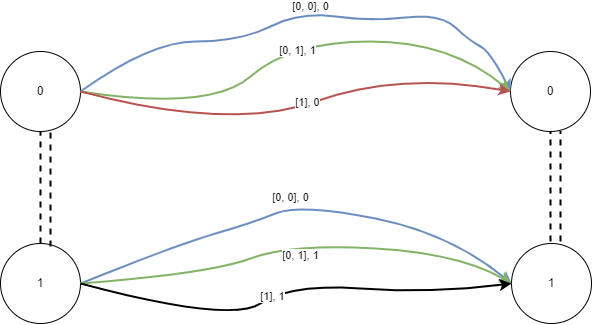
\includegraphics[scale=0.5]{templates/figures/matching-paths-rdni.png}
    \caption{There is no corresponding execution for the red and black executions.}
    \label{fig:RDNI_Matching_Paths}
\end{figure}

We formalized the notion described above to in new definition called \emph{Relatively Deterministic NonInterference} (RDNI). RDNI uses an execution relation that takes a sequence of nondeterministic events, which we call an oracle, and refers to it whenever it needs to make a nondeterministic choice (e.g. crashing or successfully executing). One important requirement is that oracle must capture all the nondeterminism in the system. If all possible nondeterminism in the system is captured by the oracle, it is possible to reason about specific sequence of nondeterministic events by reasoning about the oracle itself. This requirement is enforced by ConFrm while defining execution semantics of a language. Figure \ref{fig:RDNI_no_recovery} shows the formalization of this approach.

%% I took out users from here but will add at the end.
\begin{figure}[ht]
    \centering
    \begin{verbatim}
    Definition simple_RDNI
        {T} (p: prog T)
       (R: state -> state -> Prop) :=
      forall (o: oracle) (s1 s2: state) (res1: Result T),
        exec o s1 p res1 ->
        R s1 s2 ->
        exists res2, 
            exec o s2 p res2 /\
            R (extract_state res1) (extract_state res2) /\
            extract_ret res1 = extract_ret res2.
    \end{verbatim}
    \caption{Simple relatively deterministic noninterference.}
    \label{fig:RDNI_no_recovery}
\end{figure}

Figure \ref{fig:RDNI_no_recovery} states that a program $p$ satisfies \texttt{simple\_RDNI} for any two states $s_1$ and $s_2$ related by $R$, if there is an execution of $p$ from $s_1$ with oracle $o$ that results in $res_1$, then there is an execution of $p$ from $s_2$ with oracle $o$ that with a result $res_2$ such that, states of $res_1$ and $res_2$ are related by $R$, and return values of $res_1$ and $res_2$ are equal.

\subsection{Crash, Reboot, and Recovery}
Since we will be reasoning about crash-safe systems, RDNI should be extended to take crashes, reboots and a recovery into account. We achieve this by changing the execution semantics in the definition with one that captures the entire process of crash-reboot-recovery. There are  important differences in new execution semantics that needs to be explained. 

First is execution relation taking two program arguments, program to run and a recovery program. 

Second is how the state after a crash followed by a reboot handled. Effects of a reboot of a system may be complicated and sometimes even nondeterministic. One example of this is an asynchronous disk. When a system crashes and reboots, the disk can be in one of the multiple possible states nondeterministically due to buffered and reordered writes. To capture and quantify this source of nondeterminism, we introduce  \emph{reboot state functions} \--- or \emph{reboot functions} for short. A reboot function takes a state after a crash and returns the state that the system will be after a reboot. Reboot functions make effects of the reboot on a state deterministic, due to the fact that outcome of a function application is deterministic. Similar to the oracles, different outcomes of a nondeterministic reboot is represented by different reboot functions.

Third is that, execution semantics of a crash-reboot-recovery process must capture multiple crash and recovery attempts. One way to achieve that is providing semantics for execution of the original program followed by the multiple consecutive executions of a recovery program. Since each execution requires an oracle and each crash requires a reboot function to determine after-reboot state, new execution semantics will take a list of oracles and a list of reboot functions. We will explain further details of how executions with recovery implemented in the following section. Figure \ref{fig:RDNI_recovery} shows the formalization with recovery executions.

\begin{figure}[ht]
    \centering
    \begin{verbatim}
Definition RDNI_with_recovery
    {T} (p: prog T) 
    (rec: prog unit)
    (R: state -> state -> Prop) :=
  forall (l_o: list oracle) 
  (l_rf: list (state -> state))
  (s1 s2: state) (res1: Result T),
    exec_with_recovery l_o s1 l_rf p rec res1 ->
    R s1 s2 ->
    exists res2,
        exec_with_recovery l_o s2 l_rf p rec res2 /\
        R (extract_state res1) (extract_state res2) /\
        extract_ret res1 = extract_ret res2.
    \end{verbatim}
    \caption{RDNI with recovery executions.}
    \label{fig:RDNI_recovery}
\end{figure}

{\color{red} One paragraph explaining the changes.}


\subsection{Application specific changes}
There are some application specific changes we made to RDNI. First is the addition of a user to the execution semantics. This change allows us to model multi-user systems and discretionary access control.

Second is conditioning return value equality on a predicate for the user. This way, we can require return value equivalence to hold only for certain users, which is needed to state confidentiality of multi-user systems. For example return value equality is required when the theorem is about adversaries' executions but not needed when it is about normal user's executions.

Third is changing the definition to be about the execution of two programs instead of the same one. This change enables us to reason about functions with different input arguments, because a ConFrm program is a function and its arguments together. 
With these changes, we reach our final definition for RDNI, which is shown in Figure \ref{fig:RDNI_final}.

\begin{figure}[ht]
    \centering
    \begin{verbatim}
    Definition RDNI
        {T} (u: user) (p1 p2: prog T) 
        (rec: prog unit)
       (R: state -> state -> Prop) 
       (cond: user -> Prop):=
      forall (l_o: list oracle) (l_rf: list (state -> state))
      (s1 s2: state) (res1: Result T),
        exec_with_recovery u l_o s1 l_rf p1 rec res1 ->
        R s1 s2 ->
        exists res2,
            exec_with_recovery u l_o s2 l_rf p2 rec res2 /\
            R (extract_state res1) (extract_state res2) /\
            (cond u -> extract_ret res1 = extract_ret res2).
    \end{verbatim}
    \caption{Final definition of RDNI}
    \label{fig:RDNI_final}
\end{figure}


{\color{red}
\subsection{Termination Sensitivity}}

\section{Definitions and Meta-theory}
On top pf RDNI, ConFrm also includes structures and meta-theory that can be used to implement confidential and crash-safe storage systems. This portion consists of two parts, (1) support for abstraction, and (2) the meta-theory that provides relevant theorems to prove confidentiality of implementation from the confidentiality of abstraction. We will first present the infrastructure for defining abstractions and then explain the meta-theory.

\subsection{Abstraction Structures}
\paragraph{Cores.}
ConFrm introduces cores as the main way to model the abstract state of the system and the operations that can be performed on it. A core has four components,
\begin{enumerate}
    \item the state the system
    \item the list of possible operations that can be performed,
    \item the list of possible nondeterminism tokens,
    \item the execution semantics of each operation.
\end{enumerate}

An example core for an in-memory cache can be informally described as
\begin{enumerate}
    \item the state := a partial function from addresses to data
    \item the list of possible operations := \texttt{read}, \texttt{write}, \texttt{evict}, 
    and \texttt{flush}
    \item the list of possible nondeterminism tokens := continue execution, crash here
    \item the execution semantics of each operation := ...
\end{enumerate}.

{\color{red}Explain the example?}

Also, to ensure that tokens capture all the nondeterminism in the semantics, a proof that shows, given a token, execution semantics are deterministic is required.
  
\begin{figure}[ht]
    \centering
    \begin{verbatim}
Record Core :=
  {
    token : Type;
    state : Type;
    operation : Type -> Type;
    exec: forall T, user -> token -> state ->
        operation T -> @Result state T -> Prop;
    
    exec_deterministic_wrt_token :
      forall u o s T (p: operation T) ret1 ret2,
        exec u o s p ret1 ->
        exec u o s p ret2 ->
        ret1 = ret2;
  }.
    \end{verbatim}
    \caption{Definition of a core}
    \label{fig:Core_Definition}
\end{figure}

\paragraph{Crashes.}
ConFrm provides support for crash semantics by defining two different execution results: \texttt{Finished}, and \texttt{Crashed}. A \texttt{Finished} result means that program has successfully completed and contains a state and a return value. A \texttt{Crashed} result means that the program crashed during its execution and contains only a state, which represents the state of the system after the crash happened but before rebooting.

Crash semantics of the system are defined by the developer by defining execution rules that lead to a \texttt{Crashed} result. It is developer's responsibility to ensure that defined execution semantics correctly models the system's both normal and crash behavior.


\paragraph{Languages.}
ConFrm also includes the machinery that turns a core to a full language by equipping it with \texttt{Bind} and \texttt{Return} operations. This eliminates the repetitive work that must to be done to define languages. It also allows framework to provide core-agnostic theorems and tactics to be used in proofs.

Semantics of the language are derived from the semantics of its core. New  semantics takes a list of tokens (i.e., an oracle) and consumes exactly one at each step. 

{\color{red} Some of the Bind/Ret semantics displayed here}

ConFrm also provides some theorems regarding determinism of an execution as well as relationship between oracles and executions like how two executions relate to each other if one's oracle is a prefix of the other's.

\paragraph{Recovery semantics.}
ConFrm provides pre-defined recovery semantics for the systems and adds this semantics automatically when a language is generated from a core. To distinguish recovery semantics from the semantics of the execution of a single program, we will refer to recovery semantics as executing-with-recovery. In ConFrm's recovery model, only two outcomes are possible when executing-with-recovery: (1) execution can finish without any crashes, or (2) execution crashes then recovers after certain number of attempts. To represent these two outcomes, ConFrm uses two types of recovery result: \texttt{RFinished} and \texttt{Recovered}. \texttt{RFinished} corresponds to case (1) and \texttt{Recovered} corresponds to case (2). Since there is no rule for crashing infinitely many times, the provided semantics implicitly assume that recovery eventually will succeed. 

\begin{figure}[ht]
    \centering
    \begin{verbatim}
Inductive exec_with_recovery :
forall T, user -> list oracle -> state -> 
list (state -> state) -> prog T -> prog unit -> 
@Recovery_Result state T -> Prop :=
    | ExecFinished :
      forall T (p: prog' T) p_rec
        u o d d' t,
        exec u o d p (Finished d' t) ->
        exec_with_recovery u [o] d [] p p_rec (RFinished d' t)
    | ExecRecovered :
      forall T (p: prog' T) p_rec
        u o lo d d' get_reboot_state l_grs ret,
        exec u o d p (Crashed d') ->
        exec_with_recovery u lo (get_reboot_state d') 
            l_grs p_rec p_rec ret ->
        exec_with_recovery u (o::lo) d (get_reboot_state::l_grs) 
            p p_rec (Recovered (extract_state ret)).
    \end{verbatim}
    \caption{Recovery semantics in ConFrm}
    \label{fig:Recovery_Semantics}
\end{figure}

Figure \ref{fig:Recovery_Semantics} displays the formal definition.
Semantics for (1) is stated in \texttt{ExecFinished} rule. It is quite straightforward. If the program successfully executes, then it successfully executes-with-recovery.
Semantics for (2) is stated in \texttt{ExecRecovered} rule and more involved. It is inductively defined to capture repeated attempts of recovery until it succeeds. The rule states that, if the original program crashes, and recovery program executes-with-recovery to some result, then original program executes-with-recovery to the state of that result. Execution uses a new oracle and a new reboot function every time a crash-reboot-recovery cycle happens. Therefore, lengths of those lists implicitly determine how many times the recovery will crash until it succeeds.

\paragraph{Refinements.}
ConFrm's main mechanism for relating abstractions and implementations is refinements. 
ConFrm defines a refinement as an object between an implementation language and a core abstracting it. We extend the standard refinement definition to accommodate both crashes and oracles.

As shown in figure \label{fig:Core_Refinement_Definition}, a refinement has four components that corresponds the four components of a core, and a theorem states that a successful execution preserves the state refinement relation. The four components are
\begin{itemize}
    \item a \texttt{compile} function, that turns an  abstract operation to its implementation program,
    \item a \texttt{refines} relation that relates an abstract state to an implementation state,
    \item a \texttt{refines\_reboot} relation that relates an abstract reboot state to an implementation reboot state,
    \item and  \texttt{token\_refines} relation that relates an abstract token to an implementation oracle.
\end{itemize}

\begin{figure}[ht]
    \centering
    \begin{verbatim}
Record CoreRefinement {O_imp} (L_imp: Language O_imp) (O_abs: Core) :=
  {
    compile_core : forall T, O_abs.(Core.operation) T -> L_imp.(prog) T;
    
    refines_core: L_imp.(state) -> O_abs.(Core.state) -> Prop;
    
    refines_reboot_core: L_imp.(state) -> O_abs.(Core.state) -> Prop;
    
    token_refines: forall T, user -> L_imp.(state) -> 
        O_abs.(Core.operation) T -> (L_imp.(state) -> 
        L_imp.(state)) -> L_imp.(oracle) -> 
        O_abs.(Core.token) -> Prop;
    
    exec_compiled_preserves_refinement_finished_core :
      forall T (p2: O_abs.(Core.operation) T) o1 s1 s1' r u,
        (exists s2, refines_core s1 s2) ->
        L_imp.(exec) u o1 s1 (compile_core T p2) (Finished s1' r) ->
        (exists s2', refines_core s1' s2');
  }.
    \end{verbatim}
    \caption{Definition of a core refinement}
    \label{fig:Core_Refinement_Definition}
\end{figure}

Both \texttt{compile} and \texttt{refines} are part of the standard definition. However \texttt{refines\_reboot} and \texttt{token\_refines} relations require more explanation.

We separate \texttt{refines\_reboot} from \texttt{refines} because, in general, \texttt{refines} relation is too strong to hold for after-reboot states but we also needed a relation between them to ensure that recovery restores the original \texttt{refines} relation. {\color{red} Add example here. Cache not having latest value or smth.}

The \texttt{token\_refines} relation is more complicated. On top of the oracle and the token it relates, it takes the following parameters
\begin{itemize}
    \item a user,
    \item an implementation state,
    \item an abstract operation,
    \item and an implementation reboot function.
\end{itemize}
All these parameters are necessary to capture intricate relationship between abstract tokens and implementations' crash and recovery behavior. We can demonstrate the roles they play by examining the following example.

Assume that we are abstracting an implementation of a checksum-based log on an asynchronous disk with a \texttt{write} function.
A crash during a write to a checksum-based log may leave the log in such a state that whether the \texttt{write} succeeded or not would depends on which blocks made it to the disk before crash happened (which is determined by the after-reboot state of the implementation). In other words, success of a write after crash depends on (1) state of the disk just after the crash, and (2) state of the disk after reboot. To determine (1), we need to know the user, the starting state, and data being written, which is in the operation. To determine (2), we need to know the reboot function. Therefore, capturing the behavior of the write in this particular case requires all the parameters listed above. Other operations may require some or all of those parameters as well.

{\color{red} Maybe a figure that demonstrates above paragraph goes here.}

Similar to generating a language from a core, ConFrm can automatically generate a refinement between two languages given a core refinement between an implementation language and an abstraction core. A refinement for a language differs from a refinement for a core in three places. First, \texttt{compile} function transforms programs from the abstraction language to implementation language. Second, \texttt{token\_refines} turns into \texttt{oracle\_refines}, which relates an abstract oracle and an implementation oracle.
Third, a finished execution of any compiled program should preserve the refinement. ConFrm also provides \texttt{recovery\_oracles\_refine} relation, which relates list of implementation oracles to list of abstraction oracles by \texttt{oracle\_refines} inductively.

{\color{red} Refinement picture here.}

\paragraph{Horizontal Compositions.}
To enable modular implementations, ConFrm provides automatic derivation of a new, composite core from two given cores via horizontal composition. State of the composite core is a pair that contains the state of each the component cores. This capability allows developers to develop the system in small, self contained parts that can be combined at will when desired without much overhead. A language derived from a composite ConFrm contains support for "lifting" the programs written in a language of the one of the component cores to the language of the composite core. Similarly, it allows automatic derivation of a refinement between the two composite languages if a component of first language is a refinement of a component of the second language.


\subsection{Meta-theory}
At the heart of ConFrm lies the theorem \ref{fig:RDNI_Transfer_Definition}, which derives the confidentiality of a compiled program from the confidentiality of its abstraction. The theorem reveals sufficient conditions for preserving RDNI through refinement. The two conditions are:

\begin{enumerate}
    \item there should be a simulation between implementation and abstraction with respect to refinement relations, and
    \item if a list of implementation oracles refine a list of abstract oracles from a state with the first program, then it should refine the same oracle from any state that is equivalent to the first state with the second program.
\end{enumerate}

First condition ensures that there is no execution of a compiled program that is not captured by an execution of an abstract program. This is necessary for a property of any abstract execution to imply a property of any implementation execution. If there was an implementation execution that does not correspond to an abstract execution, then it would not be possible to reason about such execution through an abstract execution.

Second condition can be interpreted as the necessity that abstraction does not inject dependency to the confidential data into abstract oracles. Abstractions modelling some deterministic behaviors of an implementation as nondeterminism is a common pattern. For example, an abstraction of a resource allocator may model the allocation function to return an unused resource nondeterministacally, even though the implementation's behavior is actually deterministic. (e.g. returning the first available one). 

This property makes sure that developer does not abstract a behavior that depends on the confidential data in such a way. If such action would be permitted, then two implementation executions from equivalent states with the same implementation oracles could correspond to two abstraction executions with different oracles. In such a case, the noninterference of the abstraction with the same oracles wouldn't be strong enough to establish the same fact in implementation, due to the fact that noninterference of the abstraction does not state anything about executions with different oracles. Formalization of this condition can be seen in figure \ref{fig:ORS_Definition}.

{\color{red} Give example for above paragraph.}

\begin{figure}[ht]
\centering
\begin{verbatim}
Definition oracle_refines_same_from_equivalent
    (u: user) {T} (p1_abs p2_abs: L_abs.(prog) T)
    rec_abs l_get_reboot_state_imp
    (equivalent_states_abs: L_abs.(state) -> L_abs.(state) -> Prop) :=
    
forall l_o_imp l_o_abs l_o_abs' s1_imp s2_imp,

    refines_equivalent equivalent_states_abs s1_imp s2_imp ->

    recovery_oracles_refine 
        u s1_imp p1_abs rec_abs 
        l_get_reboot_state_imp 
        l_o_imp l_o_abs ->

    recovery_oracles_refine 
        u s2_imp p2_abs rec_abs 
        l_get_reboot_state_imp 
        l_o_imp l_o_abs' ->

    recovery_oracles_refine 
        u s2_imp p2_abs rec_abs 
        l_get_reboot_state_imp 
        l_o_imp l_o_abs.
\end{verbatim}
\caption{Formalization of oracle refinement being independent of confidential data}
\label{fig:ORS_Definition}
\end{figure}

\paragraph{Simulations.}
First condition states that a simulation must exist between the abstraction and the implementation. Since we introduced oracles and crash-and-recovery into execution relations, we modify the standard simulation definition to accommodate those changes. 

As shown in figure \ref{fig:Simulation_Definition}, the first change is that, modified simulation definition has three simulation relations, one for the starting states, one for the end states and one for the oracles. We separate the relation that relates the starting and end state to be able to reason about recovery where the relation that holds at the beginning and at the end are different. 

In our case, they were \texttt{refines\_reboot} and \texttt{refines} relations, respectively. However, we also define a two relation variant to use in definition  \label{fig:RDNI_Transfer_Definition}, where start and end relations are both \texttt{refines} relation.

Second change is that a simulation is defined over an entire execution-with-recovery. This allows simulation relation to be broken temporarily after a crash, as long as it is restored by the recovery process. This change is necessary because crashes may expose states that will never appear during a normal execution. This way, refinement relation can only consider the states that appear during normal execution. How to represent crash states is entirely left to the developer. 

Formal definition of a simulation can be found in figure \ref{fig:Simulation_Definition}. In implementation, we separated existence of a list of abstract oracles and existence of an abstract execution separate to shorten the proof scripts for individual theorems.   

\begin{figure}[ht]
\centering
\begin{verbatim}
Definition Simulation
   u T (p_abs: L_abs.(prog) T) (rec_abs : L_abs.(prog) unit)
   l_get_reboot_state_imp
   l_get_reboot_state_abs
   R_begin R_end :=
   
  forall l_o_imp s_imp  s_imp' s_abs,
    R_begin s_imp s_abs ->
   L_imp.(exec_with_recovery) u l_o_imp s_imp
    l_get_reboot_state_imp (R.(compile) p_abs)
    (R.(compile) rec_abs) s_imp' ->
    exists l_o_abs s_abs',
        recovery_oracles_refine u s_imp p_abs rec_abs l_get_reboot_state_imp l_o_imp l_o_abs /\
        L_abs.(exec_with_recovery) u l_o_abs s_abs l_get_reboot_state_abs p_abs rec_abs s_abs' /\
        R_end (extract_state_r s_imp') (extract_state_r s_abs') /\
        extract_ret_r s_imp' = extract_ret_r s_abs').
\end{verbatim}
\caption{ConFrm's simulation relation with oracles and execution-with-recovery}
\label{fig:Simulation_Definition}
\end{figure}


\begin{figure}[ht]
\centering
\begin{verbatim}
Lemma RDNI_transfer:
  forall O_imp O_abs (L_imp: Language O_imp) (L_abs: Language O_abs) 
    (R: Refinement L_imp L_abs)
    u T (p1_abs p2_abs: L_abs.(prog) T) rec_abs
    l_get_reboot_state_imp
    l_get_reboot_state_abs
    equivalent_states_abs cond,

    RDNI
      u p1_abs p2_abs rec_abs
      equivalent_states_abs
      cond l_get_reboot_state_abs ->
    
    Simulation R 
      u p1_abs rec_abs 
      l_get_reboot_state_imp
      l_get_reboot_state_abs ->

    Simulation R 
      u p2_abs rec_abs 
      l_get_reboot_state_imp
      l_get_reboot_state_abs ->
    
    oracle_refines_same_from_equivalent R 
      u p1_abs p2_abs rec_abs 
      l_get_reboot_state_imp 
      equivalent_states_abs ->
    
    RDNI
      u (R.(compile) p1_abs)
      (R.(compile) p2_abs)
      (R.(compile) rec_abs)
      (refines_equivalent R equivalent_states_abs)
      cond l_get_reboot_state_imp.
\end{verbatim}
\caption{RDNI transfer theorem}
\label{fig:RDNI_Transfer_Definition}
\end{figure}

%%%% SOme conclusion here
\iffalse
\section{Property Transfers}

\subsection{RDNI transfer}
- Required properties

-- SimulationForProgram
    
-- abstract oracles exist wrt (AOE)

-- oracle refines same from equivalent (ORS)

-- exec compiled preserves validity (Trivial in our case because all of our top states are valid)

-- Termination Sensitive (TS)

\subsection{ORS}
-- have same structure (program flow equivalence) (HSS)

\begin{minted}{coq}
Lemma token_refines_finished_prefix_eq:
forall ...,

token_refines u s1 op1 grs1 o1 t1 ->
token_refines u s2 op2 grs2 o2 t2 ->

exec u s1 o1 (compile op1) (Finished s1' r1) ->
exec u s2 o2 (compile op2) (Finished s2' r2) ->

have_same_structure op1 op2 -> 

(exists s1a,refines s1 s1a) ->
(exists s2a, refines s2 s2a) ->

one_prefix_of_other o1 o2 ->
o1 = o2 /\ t1 = t2.
\end{minted}

\begin{minted}{coq}
Lemma token_refines_crashed_prefix_eq:
forall ...,

token_refines u s1 op1 grs1 o1 t1 ->
token_refines u s2 op2 grs2 o2 t2 ->

exec u s1 o1 (compile op1) (Crashed s1') ->
exec u s2 o2 (compile op2) (Crashed s2') ->

have_same_structure op1 op2 -> 

(exists s1a,refines s1 s1a) ->
(exists s2a, refines s2 s2a) ->

one_prefix_of_other o1 o2 ->
t1 = t2.
\end{minted}

\begin{minted}{coq}
Lemma oracle_refines_impl_eq:
forall ...,
    oracle_refines u s1 p1 imp_reboot_f o1 oa1 ->
    oracle_refines u s2 p2 imp_reboot_f o2 oa2 ->
    
    refines s1 s1a ->
    refines s2 s2a ->
    
    exec u o1 s1 (compile p1) (Finished s1' r1) ->
    exec u o2 s2 (compile p2) (Finished s2' r2) ->
    
    have_same_structure p1 p2 u s1a s2a ->
    
    token_refines_finished_prefix_eq ->
    
    one_prefix_of_other o1 o2 ->
    not_init p1 ->
    not_init p2 ->
    
    o1 = o2 /\ oa1 = oa2.
\end{minted}

\begin{minted}{coq}
Lemma oracle_refines_independent_from_reboot_function:
forall ...,
    exec u o s (compile p) (Finished s' r) ->
    oracle_refines u s p grs o o_abs ->
    forall grs', 
      oracle_refines u s p grs' o o_abs.
\end{minted}

\begin{minted}{coq}
Lemma oracle_refines_prefix_finished_not_crashed:
forall ...,
    oracle_refines u s1 p1 imp_reboot_f o1 oa1 ->
    oracle_refines u s2 p2 imp_reboot_f o2 oa2 ->
    
    refines s1 s1a ->
    refines s2 s2a ->
    
    exec u o1 s1 (compile p1) (Finished s1' r1) ->
    exec u o2 s2 (compile p2) (Crashed s2') ->
    
    have_same_structure p1 p2 u s1a s2a ->
    
    one_prefix_of_other o1 o2 ->
    not_init p1 ->
    not_init p2 ->
    False.
\end{minted}

These are compositional in the sense that proving corresponding properties for 
each operation implies it is true for all programs created from them. 

\subsection{AOE}
\fi
\chapter{ConFs File System}
\label{chapter:ConFs}

\section{Overview}
To test the capabilities of ConFrm, we implemented ConFs, a confidential, crash-safe file system with a checksum based and encrypted log. 
ConFs is a crash-safe file system implemented in Coq and its confidentiality is proven using ConFrm framework. It has a checksum based and encrypted log, a log cache for faster log reads, a transaction system for atomic operations, two block allocators for managing data and inode blocks, and an authentication system for access control. All these components are implemented on top of each other and intermediate abstraction layers are used to provide a cleaner interface for the components above.

\section{Implementation}
We implemented ConFs as a stack of levels, each level consisting of a ConFrm layer and the programs written in that layer. This approach allows us to simplify the operational semantics as we implement higher level functionality. Each layer is designed to model how underlying implementation and hardware behaves. Using ConFrm's layer structure allow us to use the machinery and the meta-theory provided. This allowed us to encapsulate different parts of the system to only the relevant state and operations, reducing the proof effort significantly.

In the case of a layer abstracting an implementation from the level below, a simulation proof is employed to ensure that layer's semantics captures the behavior of the implementation. We will explain each level, starting from the bottom, in the following part. Figure \ref{fig:ConFs_Layers} shows how different parts of ConFs is organized.

\begin{figure}[H]
    \centering
    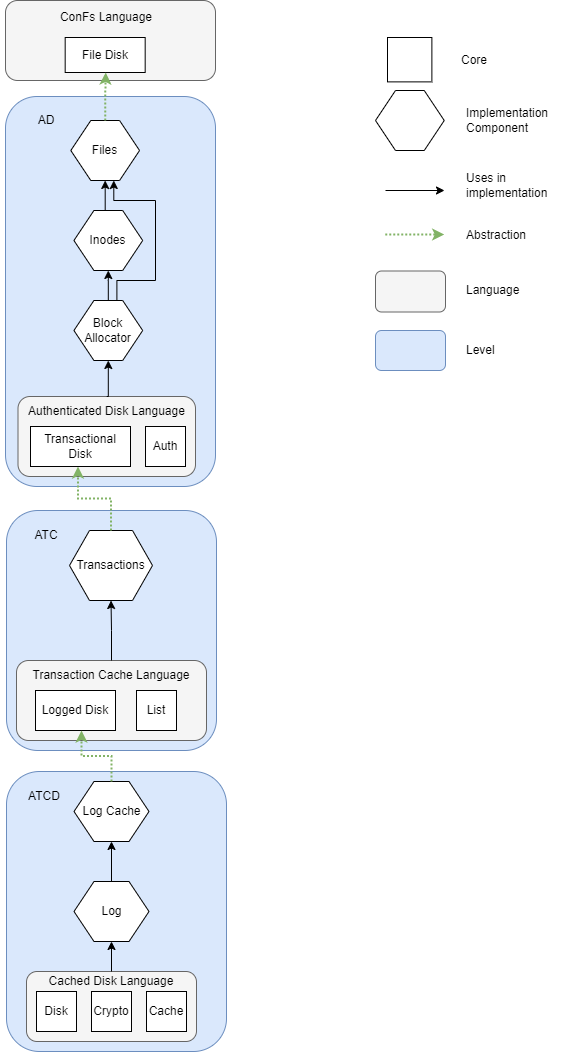
\includegraphics[scale=0.5]{templates/figures/ConFs Layers.png}
    \caption{Structure of ConFs}
    \label{fig:ConFs_Layers}
\end{figure}

\subsection{ATCD Level}
ATCD level is the lowest level of ConFs and its layer contains the model of the raw disk, a crypto engine, and in-memory data structure operations. The layer is implemented as five separate cores. These parts are disk core, crypto core, cache core, transaction list core, and the authentication core. 

Implementations in this level only uses operations from disk, crypto and cache cores; leaving transaction list and authentication cores unused. Including these cores was necessary because each file system operation will compile into a program in ATCD level and those programs will use operations from those cores. 

Thanks to the ConFrm's horizontal composition mechanism, implementations and proofs in this level uses only the relevant parts of the layer. This reduced unnecessary proof effort and implementation complexity significantly while retaining the ability to use implementations and theorems about them in the context of full level layer.

We implemented write-ahead log and log cache in this level. This level handled complicated crash and recovery semantics and presented a simple, crash-safe disk, via its representation invariant, for above levels to use. We will talk about these implementations in the following sections.


{\color{red} Table showing the state and operations of the level here}.

\subsection{ATC Level}
The level above ATCD is called ATC level and it contains a new core named logged disk that models a crash-safe disk and the possible operations on it, as well as the previously unused cores from ATCD level. ATC replaces disk, crypto, and cache cores with logged disk core. ATC also uses transaction list core, leaving authentication core unused.

Logged disk core contains an operation for each function log cache API provides. Similarly, the state of the logged disk is the crash resistant disk exposed by log cache implementation. This simplified crash semantics of the layer significantly by moving determination of possible crash states to the non-determinism tokens. This also turned its reboot and recovery semantics to a 'noop', that virtually removed the need for reasoning about the recovery process. 

\begin{figure}[H]
    \centering
\begin{verbatim}
| ExecRecover : 
      forall d u,
        exec' u Cont d Recover (Finished d tt)
        
| ExecCrashBefore :
  forall d T p u,
    exec' u CrashBefore d p (Crashed d)

| ExecCrashWriteAfter :
  forall d la lv u,
    NoDup la ->
    length la = length lv ->
    Forall (fun a => a < disk_size) la ->
    length (addr_list_to_blocks la) + length lv <= log_size ->
    exec' u CrashAfter d (Write la lv) (Crashed (upd_batch d la lv)).
\end{verbatim}
    \caption{Semantics of some of the transactional disk operations.}
    \label{fig:LD_Crash_Semantics}
\end{figure}

We implemented transactions in this level. Implementation stores active transaction in the memory as (address, block) pairs. When a transaction is committed, it deduplicates the contents based on the address - i.e. removes previous entries if an address is written multiple times in the transaction - before writing it to the log.

Implementation also enforces transaction size during a write attempt. Putting a transaction size limit allowed us to ensure that, when a transaction is committed, it will fit into the log. This design choice is made to move part of the complexity to the write function from the already complicated commit function.

{\color{red} Table showing the state and operations of the level here}.

\subsection{AD Level}
Similar to the ATC level, AD level also abstracts a part of the ATC layer. On AD level, logged disk and transaction list core is replaced with transactional disk core. ATC level's state is abstracted to a pair of disks and an indicator that stores if the transaction is empty or not. One of the disks represents the disk with active transaction applied on it. Other disk represents the disk state without the active transaction. In conjunction with transactional disk core, AD level uses authentication core to enforce access control.

Transaction being full is handled by a nondeterminism token. This abstraction allows us to remove reasoning about the precise transaction size, and turns it into a possibility that can happen in any write.

\begin{figure}[H]
    \centering
\begin{verbatim}
| ExecWrite :
  forall s a v u ,
    exec' u Cont s (Write a v) 
        (Finished (NotEmpty, ((upd (fst (snd s)) a v), snd (snd s))) (Some tt))

| ExecWriteFull :
  forall s a v u,
    exec' u TxnFull s (Write a v) 
        (Finished s None)
\end{verbatim}
    \caption{Semantics of some of the transactional disk operations.}
    \label{fig:TD_Semantics}
\end{figure}

Similar to the logged disk, if a crash happened before or after a commit is determined by a nondeterminism token. One thing to note is that rolling back to the disk without active transaction is done by the reboot function of the level.

\begin{figure}[H]
    \centering
\begin{verbatim}
| ExecCrashBefore :
  forall d T p u,
    exec' u CrashBefore d p 
        (Crashed d)

| ExecCommitCrashAfter :
  forall s u,
    exec' u CrashAfter s Commit 
        (Crashed (Empty, (fst (snd s), fst (snd s)))).
\end{verbatim}
    \caption{Transactional disk crash semantics.}
    \label{fig:TD_Crash_Semantics}
\end{figure}

Rest of the ConFs's components - i.e. block allocators, inodes and files - are implemented in this level. This level exposes the file system API.

A generic block allocator implementation is used for both inode blocks and data blocks for the files. Block allocator assumes a layout that is a single bitmap block followed by some allocatable blocks.

We implemented inodes to contain the owner of the file and a list of block numbers, which are indexes to block allocator for data blocks. There is no support for indirect blocks. ConFs stores one inode per block for simplicity.

File component uses inode functions as well as disk block allocator to implement a block based file interface. Files are represented with their inode numbers. Inode numbers are assigned by the system during file creation and returned to the user.

File component handles authentication as well as the actual manipulation of the files. Its functions are implemented as a higher-order function that handles authentication and committing or aborting, and inner functions that implements file operations.

{\color{red} Table showing the state and operations of the level here}.

\subsection{ConFs level}
ConFs level is the topmost level that provides a layer which every file system function is an operation and a state that is a mapping from inode numbers to file owner and contents. This level effectively hides all the complexities of the implementation and allows users to perceive and reason about the system similar to their intuitive understanding of it.

Inode number that is being returned upon file creation, availability of free inodes, transaction fullness, and crashes are all dictated with nondeterminism tokens.

{\color{red} Table showing the state and operations of the level here}.

% Adopted from disksec
\section{Specifiying security}
% Explains special RDNI definitions.
Security of ConFs is defined as an RDNI specification for each of the compiled FileDisk operations. In the center of these specifications is the equivalence relation between states. Since ConFs consists of four distinct levels, we had four different but related equivalence relations. We will explain these in the descending order.

\subsection{FileDisk Level Security}
We made some changes to the equivalence relation definition to unify ret\_noninterference and state\_noninterference, and to make it general enough to ensure that it can accommodate special specifications for Write and ChangeOwner operations.

We modified our equivalence relation to take an optional inode number to exclude the contents of the file that its owner is being changed.
Since equivalence relation for ChangeOwner excludes contents of the file that is being operated on, it only provides half of the required security - i.e. it excludes leakage from the changed file to the outside. The fact that no information leaks from outside to the file is covered by its functional correctness which states that file's contents stay unchanged after the operation.

\begin{figure}[H]
    \centering
\begin{verbatim}
Definition same_for_user_except (u: user) 
(exclude: option addr) (d1 d2: FD.(state)) :=
  addrs_match_exactly d1 d2 /\
  (forall inum file1 file2,
     exclude <> Some inum ->
     d1 inum = Some file1 ->
     d2 inum = Some file2 ->
     (file1.(owner) = u \/
      file2.(owner) = u) ->
     file1 = file2) /\
  (forall inum file1 file2,
     d1 inum = Some file1 ->
     d2 inum = Some file2 ->
     file1.(owner) = file2.(owner) /\ 
     length file1.(blocks) = length file2.(blocks)).
\end{verbatim}
    \caption{Equivalence relation for two FileDisk states.}
    \label{fig:eqivalence_for_filedisk}
\end{figure}


\subsection{AuthenticatedDisk and TransactionCache Level Security}
ConFrm provides a function that converts an equivalence over abstract states to an equivalence over implementation states given that a refinement between two exists. Informally, function states that two implementation states are equivalent if there exists two equivalent abstract states that are refined by the implementation states.

\begin{figure}[H]
    \centering
\begin{verbatim}
Definition refines_related 
 (related_abs:  L_abs.(state) -> L_abs.(state) -> Prop)
 (si1 si2: L_imp.(state)) : Prop :=
exists (sa1 sa2: L_abs.(state)),
  R.(refines) si1 sa1 /\
  R.(refines) si2 sa2 /\
  related_abs sa1 sa2.
\end{verbatim}
    \caption{Equivalence conversion function from ConFrm}
    \label{fig:refines_related}
\end{figure}

This function alone was sufficient derive the equivalence for these two levels. However, this is not generally is the case. Sometimes, extra conditions are needed to establish the relation between the parts of the implementation state that is abstracted away. We will present examples of such instances in the following section.

Main reason for this is that, oracles in ConFrm implicitly dictates number of execution steps a program takes. Semantics of a program requires consumption of an exactly one token per operation executed. This requirement generally implies two noninterfering programs have to follow the same execution paths. 

%%%% ADD an example noninterference spec here?

\subsection{CachedDisk Level Security}
{\color{red} INTRO HERE}

Consider the following read function:

\begin{figure}[H]
    \centering
\begin{verbatim}
Definition read a :=
  mv <- Cache_Read a;
  if mv = Some v then 
    Ret v
  else
    Disk_Read a
\end{verbatim}
    \label{fig:refines_related}
\end{figure}
%
Proving noninterference of this function requires showing that if there is an execution of the function from a state with a particular oracle, then there must be an execution from a related state with the same oracle. Since having same oracle dictates that programs have to follow the same execution paths, two related states have to contain exactly same addresses in their caches (corresponding data could be different).

If an abstraction of the states hides the existence of a cache, then refining two related abstract states is not sufficient to capture this requirement. In this instance, equivalence relation needs to be supplemented with this property to make it finer-grained.

This particular example and some other more complicated variants are present in log functions. Therefore, we supplemented the equivalence relation with the following:

{\color{red} Property here}

{\color{red} Explanation of the property here}


\section{Proving security}
We proved confidentiality of ConFs with two general categories of theorems: (1) confidentiality proofs of FileDisk operations, and (2) premises required to establish confidentiality of the refining programs of the operations. Proving (1) was relatively easy thanks to the simple structure of FileDisk state and semantics. Majority of the effort among them went into proving (2).

Proving (2) required us to prove 2 different properties for each operation: (a) oracle refinement being independent of confidential data, and (b) existence of a refined abstract oracle. Proofs in a compositional manner - i.e. corresponding properties are proved for each operation of each layer, then brought together to construct required proofs. Compositional nature of the properties significantly reduced the proof effort and repetition between layers.

One interesting case appeared regarding write operations that overwrite some data with itself. Possibility of such operations made it impossible to determine if a write succeeded or not after a crash by just examining the disk's final state. To resolve this problem, we had to reason about precise number of steps the function ran as well as the required conditions on the crash and reboot states of the disk after the execution.  This precise and low level reasoning was tedious and required significant proof effort. Despite our best efforts, question of whether this can be solved at meta-theoretic level or with another proof strategy that requires less effort remains open.

During this reasoning, we had to employ the condition that, in the log, current and residual blocks at the same address can't be identical. Encryption of each block ensured that such a condition is exponentially unlikely. By design, since a residual block and a current block cannot belong to the same transaction, they must be encrypted with different keys. Therefore such a condition does not weaken the conclusion significantly.


{\color{red} Termination Sensitivity may go here. Maybe an explanation of why it was as hard as it is?}


\chapter{Evaluation}
This section experimentally answers the following questions:

\begin{itemize}

\item
  Is our confidentiality specifications trustworthy?  That is, are noninterference theorems sufficient for applications to prove confidentiality of their own data?
  What assumptions do these proofs rely on?

\item
  How much effort was required to develop the frameworks, and to use frameworks to prove the security of the systems?

\item 
  How are the performances of the systems compare to existing ones?
  %How much runtime overhead does DiskSec's approach impose in SFSCQ?
\end{itemize}

\subsection{Specification trustworthiness}

To evaluate the trustworthiness of SFSCQ's specifications, we performed several
analyses.


\paragraph{End-to-end application confidentiality.}

To demonstrate that SFSCQ's specifications capture confidentiality in
a useful way, we developed a simple application on top of SFSCQ that
copies a file, wrote a confidentiality specification for this application
(namely, that the application does not leak the data of the copied
file), and proved it.  This application tests two aspects of SFSCQ's
specs.  The first is, does SFSCQ's specification actually guarantee
confidentiality?  The second has to do with SFSCQ's discretionary access
control model: can application developers demonstrate that they are not
inadvertently leaking data, despite having the discretion to do so?

We were able to prove the correctness and security of our implementation
of \texttt{cp}.  This suggests that SFSCQ's specifications capture sufficient
information for \texttt{cp} to conclude that its data remains confidential,
and that it is possible for application developers to show that they do
not abuse their discretionary privileges by leaking data.


\paragraph{Bug case study.}

To evaluate whether SFSCQ's specifications would eliminate real
security bugs, we qualitatively analyzed the bugs presented in
\ref{s:motivation} to determine whether SFSCQ's theorems preclude
the possibility of that bug.  \ref{fig:bugs-addressed} shows the
results.  Functional correctness theorems preclude the possibility of
integrity bugs.  DiskSec state noninterference precludes the possibility
of all confidentiality bugs in our study.  No bugs were prevented by
return-value noninterference, because return-value noninterference captures a
particularly simple kind of bug, such as the file system forgetting
to check the ACL on \texttt{open()}.  No file-system developers made this
mistake in our study.  Nonetheless, return noninterference is important
for completeness of SFSCQ's theorems.  Overall, the results demonstrate
that SFSCQ's theorems preclude the possibility of all studied bugs.

\begin{figure}[ht]
  \centering
  \small
  \begin{tabular}{@{}p{2.4in}p{0.5in}@{}}
    %\toprule
    %\multirow{2}{*}{\textbf{Description}} & \textbf{Theorem} \\ & \textbf{violated} \\
    %\midrule
    anyone can change POSIX ACLs~\cite{CVE-2010-2071, CVE-2010-1641, CVE-2016-1237} & state NI \\
    reiserfs permissions can be changed \\ \quad by writing to hidden file~\cite{CVE-2010-1146} & state NI \\
    truncated data can be accessed~\cite{CVE-2015-8374}
                         & state NI \\
    crash can expose deleted data in ext4~\cite{CVE-2017-7495} & state NI \\
    crash can expose data in ext4~\cite{git:469017} & state NI \\
    can overwrite append-only file in ext4, btrfs~\cite{CVE-2010-2066, CVE-2010-2537} & integrity \\
    can overwrite arbitrary files in ext4~\cite{CVE-2009-4131} & integrity \\
    % SGID directories can become writeable in overlayfs~\cite{CVE-2016-1575} &
    % write confidentiality, but \emph{N/A}\footnote{any SGID, writeable
    % directory violates write confidentiality, but no support or model of
    % SUID/SGID} \\
    %\bottomrule
  \end{tabular}
  \caption{Security bugs in Linux file systems and which SFSCQ theorem precludes them.}
  \label{fig:bugs-addressed}
\end{figure}


\paragraph{Trusted computing base.}

Both systems assume the correctness of several components.  They assume
that Coq's proof checking kernel is correct, because it verifies
the proofs. Both systems assume that the Haskell runtime and support
libraries (and the underlying Linux kernel) do not have bugs, since
they generate executable code through extraction to Haskell. Both systems
assume that their respective framework's model of the disk is accurate.  In particular, all
non-determinism in the oracles and execution semantics must be ``realizable,''
in the sense that it is actually possible for an execution to observe
all specified non-determinism (e.g., crashing at any point), and this
non-determinism must be independent of confidential data.  All proofs in the frameworks and the systems are checked by Coq proof assistant.


\subsection{Effort}

% these numbers were computed by the scripts in
% osdi18-security/effort-estimate/; see the README.md there for details.

To understand how much effort was required to verify DiskSec and SFSCQ, we
compared SFSCQ to the implementation of DFSCQ on which SFSCQ is based.
\ref{fig:loc} shows the results (counting the sum of lines removed and lines
added), breaking down the differences into several categories.  The core
infrastructure, including improvements to DFSCQ's CHL, amounted to around
9,300 lines.  We made significant changes to DFSCQ to develop SFSCQ, but many
of these changes were mechanical fixes to proofs to address small changes. In
addition, using DiskSec in SFSCQ required around 1,900 lines of new code and proofs.
Porting DFSCQ to the first version of DiskSec (without support for changing
permissions) took one author about 3 months, and another 2 months to
mostly finish support for permission changes.

\begin{figure}[ht]
  \centering
  \begin{tabular}{lr}
    %\toprule
    \textbf{Component} & \textbf{Changes to DFSCQ} \\
    %\midrule
    DiskSec & 9,283 \\
    DFSCQ proof fixes & $-10,471$, $+26,433$ \\
    & \quad (36,094 total) \\
    SFSCQ impl.\ and proofs & 1,837 \\
    Verified \texttt{cp} application & 407 \\
    %\bottomrule
  \end{tabular}
  \caption{Lines of code change required to implement DiskSec and apply it to build
    SFSCQ. Counts measure the diff between DFSCQ and SFSCQ.}
  \label{fig:loc}
\end{figure}


\subsection{Performance}

We expect that the performance overhead of DiskSec is nearly zero, because
most of its code changes (such as handles, sealing, and unsealing) are
eliminated in the process of generating executable code.  (All of the
Seal and Unseal operations turn into \texttt{return} statements.)  The only
exception is checking permissions when reading data from a file; the
original DFSCQ implementation had no permission checks, which we added
in SFSCQ.

To check that DiskSec introduces almost no overhead,
we used two microbenchmarks (LFS smallfile and largefile
benchmarks~\cite{rosenblum:lfs} as modified by DFSCQ~\cite{chen:dfscq}).
As a baseline, we compare with two versions of DFSCQ, on which SFSCQ
is based.  The first is unmodified DFSCQ\@.  The second is a version of
DFSCQ with a two-disk-barrier write-ahead log (instead of its default
checksum-based log).  This matches the modification we made to SFSCQ, as
mentioned in \ref{s:fs:impl}.  For comparison with other file systems,
such as Linux ext4, we refer the reader to the detailed evaluation in
the DFSCQ paper~\cite[\S 7.4]{chen:dfscq}.

\ref{fig:perf} shows the results, which confirm that SFSCQ performs
nearly identically to DFSCQ in the same logging configuration.  The use
of a two-disk-barrier write-ahead log incurs some performance overhead
for smallfile; largefile performance is not impacted because its file
data writes bypass the log.

\begin{figure}[ht]
  \centering
  \begin{tabular}{lrr}
    %\toprule
    \textbf{Filesystem} & \textbf{smallfile} & \textbf{largefile} \\
    %\midrule
    DFSCQ & 446 files/s & 108 MB/s \\
    DFSCQ (no checksums) & 295 files/s & 109 MB/s \\
    SFSCQ & 299 files/s & 100 MB/s \\
    %\bottomrule
  \end{tabular}
  \caption{Benchmarks showing performance of SFSCQ compared to DFSCQ and a
    version of DFSCQ with a comparable logging implementation.  Numbers
    shown are the median of 30 runs.}
  \label{fig:perf}
\end{figure}

\chapter{Conclusion}
\appendix
\chapter{Tables}

\begin{table}
\caption{Armadillos}
\label{arm:table}
\begin{center}
\begin{tabular}{||l|l||}\hline
Armadillos & are \\\hline
our	   & friends \\\hline
\end{tabular}
\end{center}
\end{table}

\clearpage
\newpage

\chapter{Figures}

\vspace*{-3in}

\begin{figure}
\vspace{2.4in}
\caption{Armadillo slaying lawyer.}
\label{arm:fig1}
\end{figure}
\clearpage
\newpage

\begin{figure}
\vspace{2.4in}
\caption{Armadillo eradicating national debt.}
\label{arm:fig2}
\end{figure}
\clearpage
\newpage

%% This defines the bibliography file (main.bib) and the bibliography style.
%% If you want to create a bibliography file by hand, change the contents of
%% this file to a `thebibliography' environment.  For more information 
%% see section 4.3 of the LaTeX manual.
\begin{singlespace}
\bibliography{main}
\bibliographystyle{plain}
\end{singlespace}

\end{document}

